% \section{Introduction}
% Todo: Introduction structure
% 0) we introduce & define the problem 1) we survey which techniques
% exist 2) we implement (for a lack of readily available implementations)
% and compare the most promising ones 3) we draw conclusions for when to
% use which technique


% TODO: Include term predictive CI, link to FB paper and
%https://www-sciencedirect-com.tudelft.idm.oclc.org/science/article/pii/S0164121218301730

% TODO: What about the alternate solution, installing plugins to report
% precise data? Ie., maven plugins
% - Lots of effort
% - not a generic solution
% - how to analyze history where such plugins were not installed
% - unclear which information you want

% TODO It would be futile to compare our techniques with one of the
% existing manual regex parsers, as (a) as our literature survey showed,
% their scope is mainly limited to the Java ecosystem and (b) whether
% they would work or not would be randomly based on whether the project
% we select exhibits features their regular expressions were trained for.
% Finally, they are not really automatic

\lstset{
  morekeywords={},
	basicstyle=\ttfamily\scriptsize,
  postbreak=\mbox{\textcolor{blue}{$\hookrightarrow$}\space},
  showspaces=false,
  showstringspaces=false,
  stringstyle=\color{Plum},
	frame=single,
  extendedchars=false,
  texcl=false,
  aboveskip=\baselineskip,
  belowskip=0pt
}

Within the past two decades, Continuous Integration (CI) has become a
ubiquitous best practice to streamline the build process of software
projects~\cite{hilton2016usage,beller2017oops,staahl2014modeling}.
Build logs are a textual by-product that automatic software build
processes create.
As a treasure trove of information~\cite{meyer},
build logs contain trace outputs of not only the elementary steps to
``make'' a project---such as retrieving and resolving dependencies and
compiling---but also about ancillary quality assurance steps---such as
testing the software and running automated static analysis tools.
The
contents of build logs can be highly variable depending on which tools
are involved in the build process and how they are
configured.
The format of logs changes as projects and build tools evolve over time.
Typically, though, they are at least a semi-structured and
somewhat stable journal of the commands executed during the build and
their results.

When a build or one of its steps fails, developers typically
scavenge the logs for information related to the source of the error.
This manual activity is
tedious and prone to error~\cite{santolucito2018statically}.
As a
single build log can be over 50 megabytes large~\cite{beller2017oops},
finding the small chunk of information in it which is linked to the error,
is akin to searching for a
needle in a haystack.
In addition to helping understand and fix build failures, the information
richness of build logs enables a plethora of other applications: with
the help of
build logs, we can better understand and categorize CI
failures and compile
errors~\cite{islam2017insights,seo2014programmers}, differentiate
testing practices~\cite{orellana2017differences,vassallo2017a-tale},
train classifiers to predict the build outcome and
duration~\cite{ni2017cost,bisong2017built,machalica2019predictive}, or
investigate static analysis tools in CI
builds~\cite{zampetti2017open}.

However, manual analysis of build logs does not
scale to the number of build logs and amount of information that such
sophisticated applications require.
Moreover, being able to
automatically extract relevant pieces of information from build logs
can also help
developers debug a broken build more quickly without having to browse
the entire build log.

\begin{figure*}[htb]
	\centering
	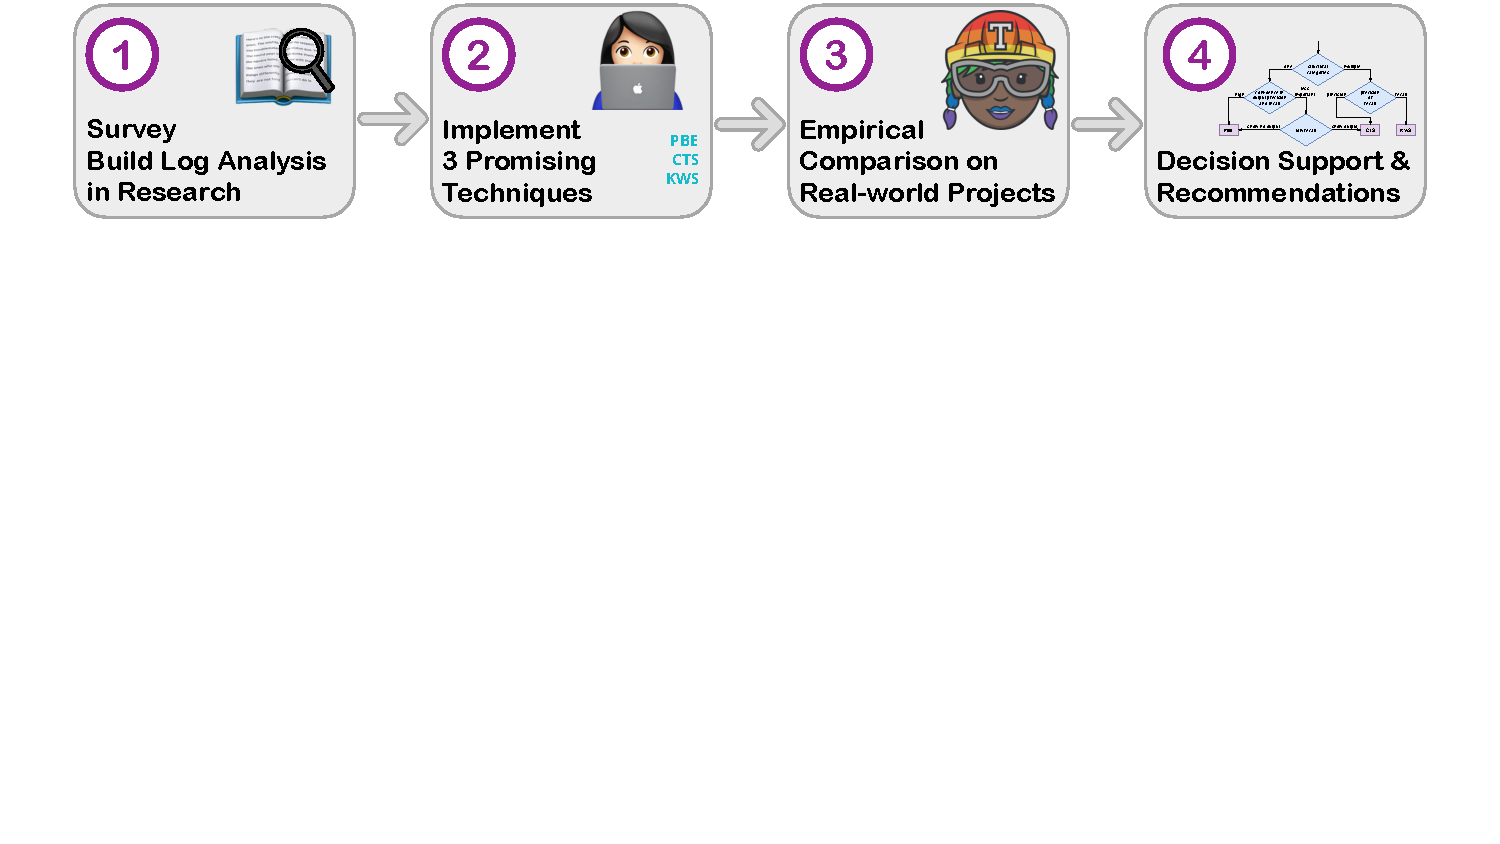
\includegraphics[width=\textwidth, trim={1.2cm 10.5cm 1.2cm 0cm},
	clip]{img/overview.pdf}
	\caption{Research Design.}
	\label{fig:overview}
\end{figure*}

Despite its central role for helping developers and the enablement of
on-ward applications of build logs, the process of how to
automatically analyze build logs has thus far received little
attention as a separate research topic, bringing us to our first
research question:
\begin{simplebox}[minipage boxed title*=-5cm]{\textbf{Research Question
1}}
What are the state-of-the-research techniques to analyze build logs?
\end{simplebox}

To answer this question, we start our investigation by performing an
extensive literature study (\Cref{fig:overview}).
It shows that
less than half of the 61 works which rely on build log analysis
describe in detail how they performed it, and even fewer
made their implementation available.
The literature
survey identifies three prevalent strategies to
analyze build logs: Using 1) a set of
manually curated regular expressions,
similar to TravisTorrent~\cite{beller2017oops},
2) information
retrieval techniques,
% TODO: Can you shortly explain the technique here?
and 3) a list of search keywords
to identify regions of interest in the build log.

Even though these three approaches to retrieve information chunks from
build logs have different strengths and weaknesses, the literature
survey shows that their use often seems arbitrary.
As a consequence,
in RQ2 we ask:

\begin{simplebox}[minipage boxed title*=-5cm]{\textbf{Research Question
2}}
What are the comparative strengths and weaknesses
of promising build log analysis techniques?
\end{simplebox}

To answer this question, in the second step of our study
(\Cref{fig:overview}), we build and compare three
implementations that each stand protoypical for one of the idenitied
strategies to analyze build logs:

\begin{itemize}
  \item \textbf{Program Synthesis by Example (referred to as PBE)}
  Based on manually supplied example pairs of build logs and chunks,
  PBE automatically
  synthesizes
  a regular expression extracting the given chunks within the build logs.
  \item \textbf{Common Text Similarity (CTS)}
  % TODO what is the vector space model?
  Using the Vector Space Model, CTS selects lines of a log which are
  most similar to the lines present in manually supplied example chunks.
  \item \textbf{Keyword Search (KWS)}
  % TODO what is an ad-hoc method?
  Ad-hoc method for finding fitting passages by searching the whole
  text of a build log for
  the occurrence of specific trigger words.
\end{itemize}


In the third step, we conduct an empirical study to gauge the performance
of
these chunk retrieval techniques in
real-world projects under a variety of conditions.
Our study is based on the \emph{LogChunks} data
set~\cite{brandt2020logchunks}, which encompasses build logs from
80 popular open-source projects and a broad range of different
build tools and programming languages.

Finally, we develop a set of guidelines (step 4) on how to choose a
technique given a goal.
We recommend PBE for use cases where the desired information is always
represented in the same structural way and high confidence in
precision and recall of the chunk retrieval is required.
Results
produced by PBE are suited for automatic on-ward processing.
CTS is
well-suited when the representation of the desired information varies
slightly and the output of the chunk retrieval is further processed by
a human.
In cases where the textual representation of the desired
information in the log is unpredictable or varies greatly, KWS seems
to be the best choice.
However, its low precision---it extracts a
context of multiple lines around a finding---makes it generally
unsuited for automatic on-ward processing and instead requires a human
to further inspect and interpret the output chunk.
A hybrid-solution combining the three techniques might be the best
allround solution.

In short, this article contributes
\begin{itemize}
\item the first systematic study of the emerging field of build log
analysis.
\item three prototypical open-sourced implementations of the most
promising chunk retrieval techniques.
\item a large empirical study comparing the three techniques.
\item systematic guidelines on when to use which technique.
\item a detailed replication package~\cite{brandt2020chunk-replication}.
\end{itemize}

\section{Systematic Literature Mapping Survey}
\label{sec:survey}

In this section, we survey the emerging field of build log
analysis.
We first start with a differentiation to the related field of general
system log analysis.
Then, we describe the methodology and results of a systematic mapping
study to
determine the state-of-research on build log analysis following the
guidelines by Petersen et
al.~\cite{petersen2008systematic,petersen2015guidelines}.

We close by summarizing how build logs are commonly
analyzed in literature and discuss the implications of these findings.

\begin{figure}[tb]
	\centering
	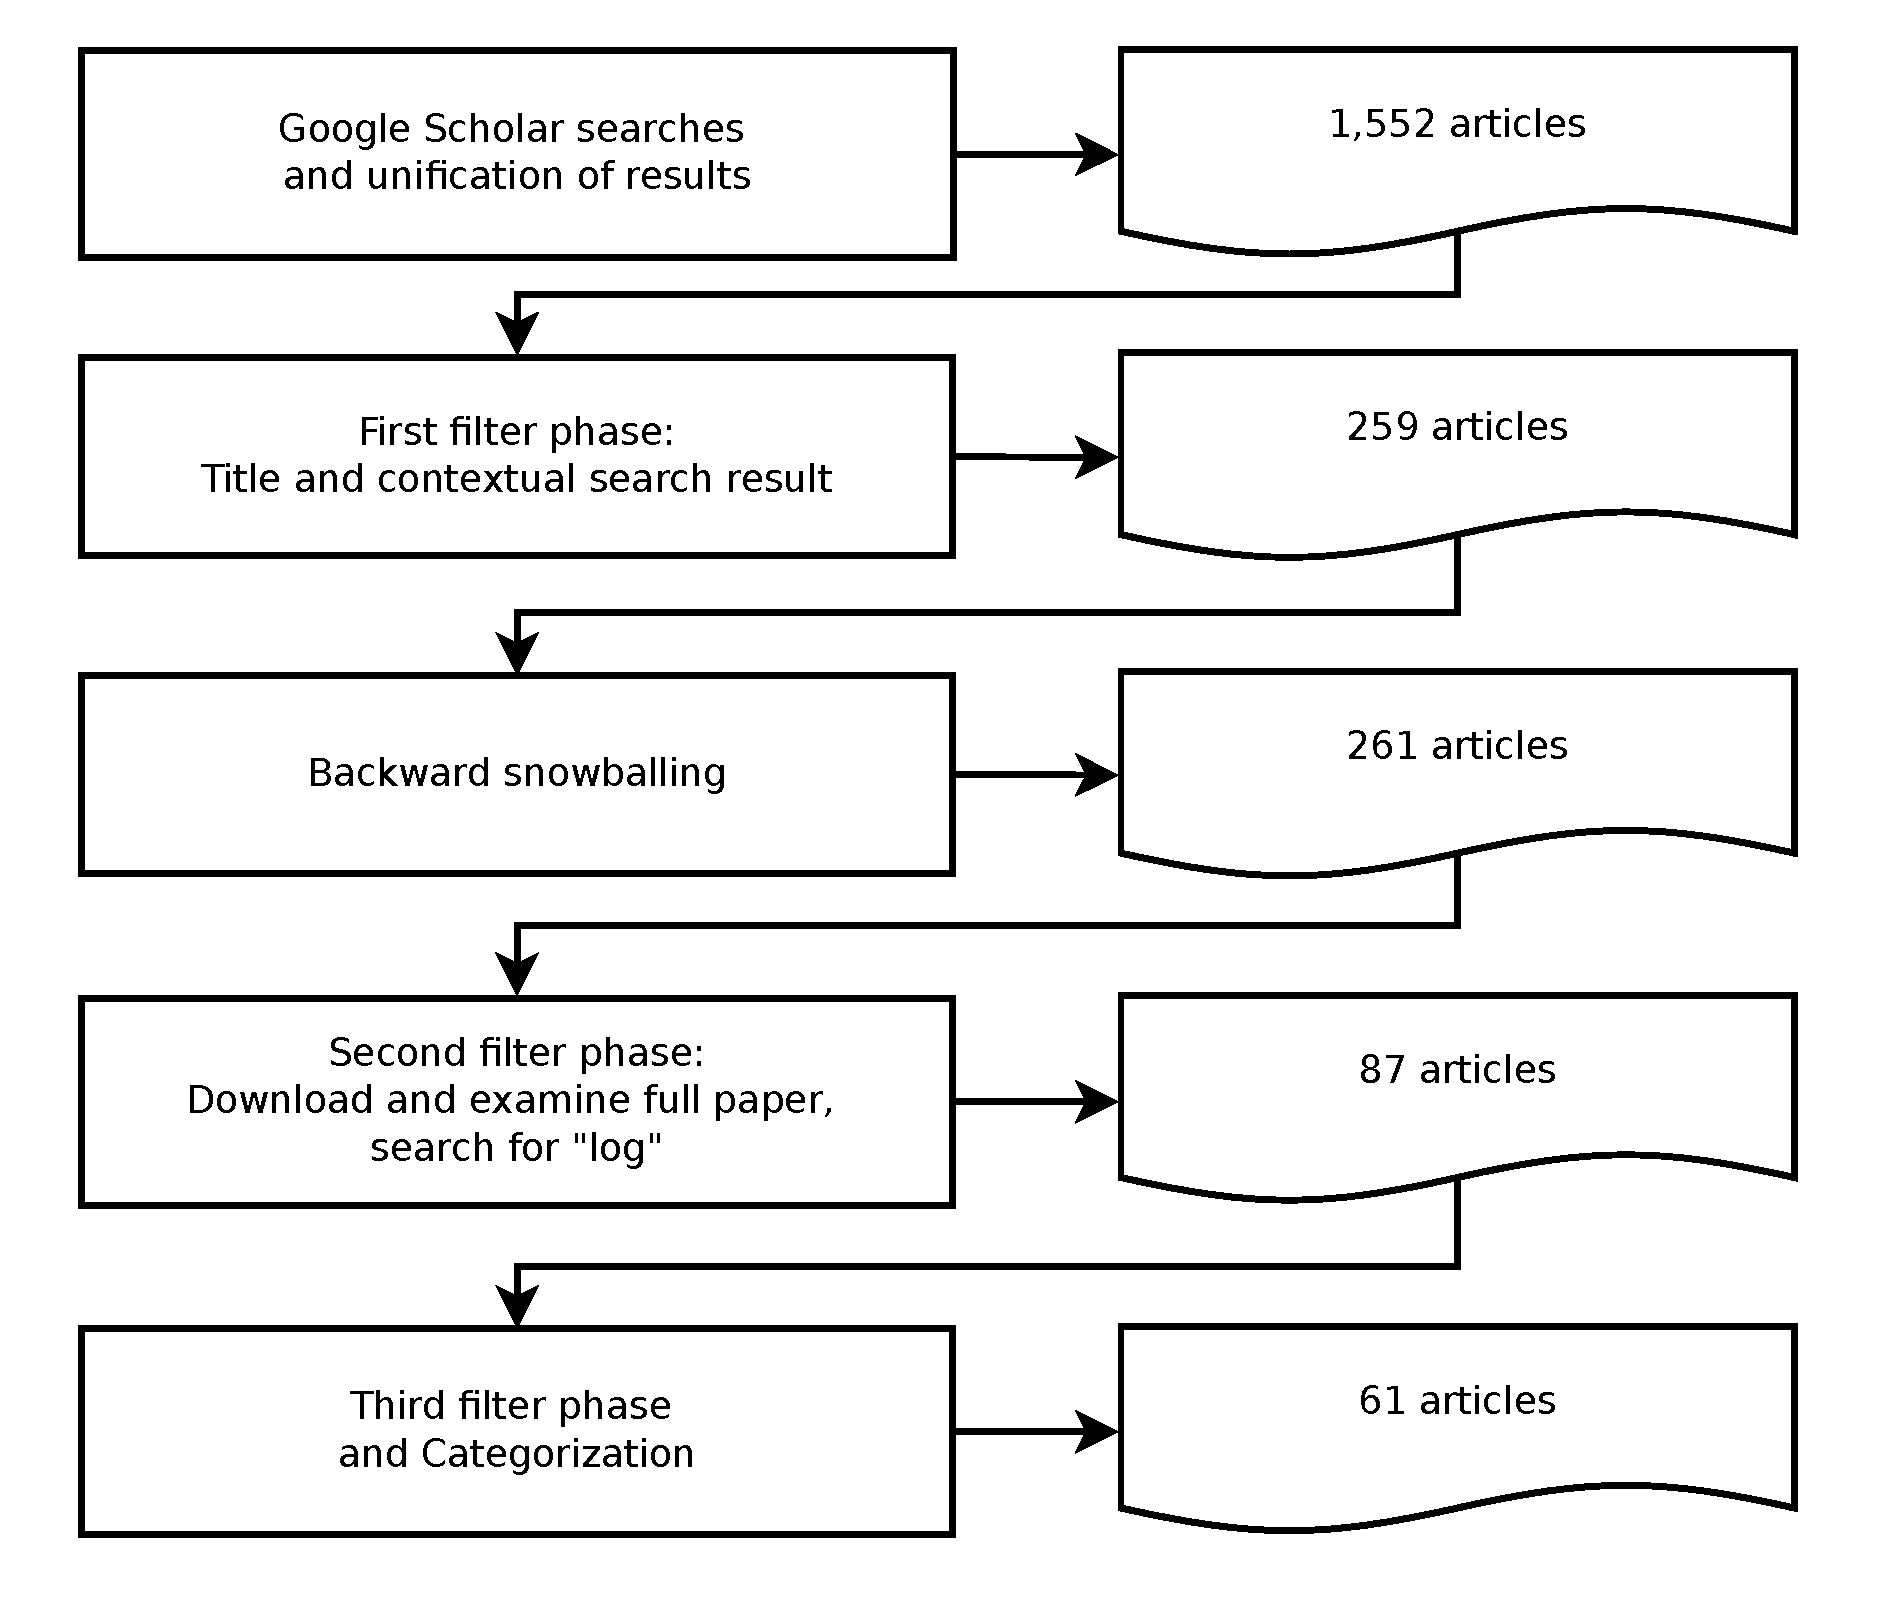
\includegraphics[width=\columnwidth, clip]{img/lit_survey.pdf}
	\caption{Literature selection process, following
	\cite{petersen2015guidelines}.}
	\label{fig:lit-survey}
\end{figure}


\lstset{
  morekeywords={INFO, WARN, 2008, 11, 09},
  alsoletter=-20819,
  keywordstyle=\bfseries\color{Plum},
  escapeinside=**
}
\begin{figure}[b]
  \centering
  \lstinputlisting[breaklines=true]{listings/syslog.txt}
  \caption{System Log excerpt.
Example adapted from~\cite{he2017towards}.}
  \label{lst:system-log}
\end{figure}

\subsection{Distinction from System Log Analysis}
\label{sec:system-log-analysis}
A field related to build log analysis is the processing of system logs produced during runtime of the system.
The first difference here is that build logs are produced during runtime
of the build of the system, not the system itself.
In terms of the contents of the logs, the main difference is that system
logs are fundamentally structured
through events.
Each line in a log file represents one event with a
set of fields: timestamp, verbosity level and raw message
content~\cite{he2017towards}.
\Cref{lst:system-log} shows
example lines from a system log.


The first goal in analyzing system log files is generally to
separate constant and variable parts within a log
message~\cite{nagappan2010abstracting,he2017towards}.
Next, the log
messages are clustered into log events, unifying messages with
identical constant parts and varying parameters.
Then, a log parser works on this intermediate representation.
Its output is an ordered list of timed events and their corresponding
parameter values~\cite{he2016evaluation}.
This structured log can serve as input to various machine learning and
data mining processes.

In principle, one can apply the techniques developed for system log
analysis
to parts of the build logs that have this same structure.
% TODO this explanation is not understandable.
It needs to better embedded in the surrounding text
One example is comparing execution traces to reference
traces of intended behavior to detect anomalies.
Amar et
al.~\cite{amar2019mining} employed a similar approach to detect
relevant lines in build logs.
However, almost all of the techniques developed to analyze system logs
leverage their inherent event structure.
Build logs generally lack this structure and thus require different
bespoke approaches.
% In this article, we focus on extracting a single specified information
% from the build log as a whole with chunk retrieval techniques.
% Chunk
% retrieval techniques are used as a part of log parsing to retrieve the
% values of variable parts in a log message, e.g.\ by using regular
% expressions~\cite{nagappan2010abstracting,xu2009detecting}.


\subsection{Study Selection}
\Cref{fig:lit-survey} presents an overview of our study selection
process.
Since the field of build log analysis is relatively young, we
surveyed as broad a population of scientific material as possible.
We did not limit our sources to specific Software Engineering
venues~\cite{petersen2015guidelines}, but survey all sources
monitored by Google Scholar, including Bachelor's and Master's
theses and academic slide decks.
We use Google Scholar as opposed to Scopus or
other databases because it is the search engine for academic articles with
the broadest and most current index, including preprints.

An initial Google Scholar search for variations of ``build log''
returned more than 2.2 million results (2020-03-15), many of which stem
from unrelated fields such as construction and wood working.
We refined our search criteria to exclude such obvious
non-related fields and also to exclude works on systems
or event logs (see \Cref{sec:system-log-analysis}).
This left us with 1,552 search results
(2020-03-15).
Our replication package documents the full search
queries~\cite{brandt2020chunk-replication}.
To make handling so many search results feasible, we employed a
three-pass filtering strategy:

First, we filtered articles based on (a) their title and (b) the
contextual information Google Scholar displayed.
We included works at large that seemed to bear a resemblence to software
engineering and building software.
We excluded wroks written in a language unintelligible to the authors
(i.e., not English or German), which disregarded fewer than 1\% of search
hits.
We then unified
the results of the four search queries based on the link as the
identifying element, removing 60 articles that appeared in more than
one search query.
We removed further duplicates based on the title and were
left with 256 (16\%) of the original search results.
% removed duplicates of data extraction pass already here
With these 256 remaining articles, we followed a backward snowball
sampling for related work.
If an article referenced a new work in the context
of build log analysis, we added the new one to our literature set.
This added five articles (eight before
duplicate elimination), leading to a total of 261
works.


Subsequently, we performed a second, finer filter phase by downloading the
full text of the works, reading their abstracts, and searching the
full text
for the occurrence of ``log.''
If a work showed traces of
working with build logs, we included it in our survey.
In total, we
were left with 87 works after the second filtering phases.

\subsection{Article Classification}
Having trimmed down the set of articles by 95\%, we investigated the
remaining ones in depth.
We wanted to characterize how research uses build logs.

% TODO (resolved): RQs mentioned before explicitly stated
Specifically, we were interested in
\begin{itemize}
  \item what information is retrieved from the logs and
  what the retrieved information is used for (\textbf{RQ1.1})
  \item which techniques are used to process the build logs,
  in how much detail they are described, and whether they are published
  as tools (\textbf{RQ1.2})
  \item what kind of build logs are used and the origin of these
  logs.
(\textbf{RQ1.3})
\end{itemize}

This lead us to the following research questions:
\begin{simplebox}[attach boxed title to top center={yshift=-6mm}]
{\textbf{RQ1:} What are the state-of-the-research
techniques to analyze build logs?}
\begin{itemize}[leftmargin=2cm]
  \item[\textbf{RQ1.1:}] Which information is targeted?
  \item[\textbf{RQ1.2:}] Which techniques are used?
  \item[\textbf{RQ1.3:}] Which build logs are analyzed?
\end{itemize}
\end{simplebox}

Since we had been careful to include rather than exclude borderline
works, this deeper evaluation excluded another 15 articles from the 87
works left after the second filter phase.
Multiple articles were extensions of others.
Of these, we only considered the earliest article which reported on
the processing of build logs.
This excluded another 11 articles.
In sum, we extracted data from 61 articles.

To guide the data extraction we created a template.
The template form contained questions to answer RQ 1.1 through RQ 1.3,
for example ``Is the technique explained in sufficient detail?'' and
``What is the source of the build logs?'' As recommended by Petersen et
al.~\cite{petersen2015guidelines}, we started the mapping study with a
pilot study:
both authors extracted	data from the same five articles and held a
consensus meeting to unify their understanding
of the data extraction template.
We divided the remaining 46 articles evenly between the two authors
and inspected them as closely as necessary to fill out the template
with confidence,
starting from occurrences of ``log'' or ``build'' within the article's
text.
For questions that did not require a boolean answer, we allowed assigning
multiple tags or categories as the first part (``preparation phase'')
of a virtual open card sorting~\cite{zimmermann2016card}.

% TODO: add more concrete example, such as use of retrieved x: developer
feedback, build data set
Once we had classified all works, we went into the second phase
(``execution phase'') in which we  grouped tags
together and found synonyms.

%The full data extraction template and our results of this step can be
%found in our replication package~\cite{brandt2020chunk-replication}.


% TODO (resolved): RQs just appeared unconnected out of the blue


% TODO: vertical alignment of rows with text to middle so they are aligned with pictograms on the right?
\addtolength{\tabcolsep}{-5pt}
\begin{table*}[tbhp]
\tinyish
\centering
\caption{Overview of build log analysis techniques.}
\begin{tabularx}{\textwidth}{@{}lXl@{}}
\toprule
Name			     & Sources	& Frequency	  \\
\midrule
Parser	&
\cite{vassallo2018un-break,zhang2016android,seo2014programmers,hassan2019tackling,hassan2017automatic,chromy2007integration,mesbah2019deepdelta,wen2018blimp,kwon2018prioritizing,adams2007design,rahman2018impact,brandyberry2006continuous,tomassi2019bugswarm,ren2018automated,vassallo2019automated,cavalcanti2019impact,sippola2013qt,felipe2012towards,shi2018evaluating,urli2018design,selberg2012use}
&

\includegraphics[width=0.55\columnwidth]{img/lit-sur/techniques-no-guidelines-cropped_21.pdf}
\\
Regular expression
&\cite{beller2017oops,hassan2017change,macho2018automatically,vassallo2017a-tale,lou2019history,hassan2017automatic,rott2019empirische,zampetti2019study,zhao2018comparing,rausch2017empirical,ghaleb2019studying,zampetti2017open,zhang2019large,kavaler2019tool,morris2010experience}
&

\includegraphics[width=0.55\columnwidth]{img/lit-sur/techniques-no-guidelines-cropped_15.pdf}
\\
Manual inspection  &
\cite{sulir2016quantitative,hassan2017automatic,bouabana2019theory,barinov2017applying,silva2018build,ghaleb2019empirical,marcozzi2019systematic,hukkanen2015adopting,rausch2017empirical,hassan2017mining,zolfagharinia2017not,cassee2019impact}
&

\includegraphics[width=0.55\columnwidth]{img/lit-sur/techniques-no-guidelines-cropped_12.pdf}
\\
Machine Learning  &
\cite{hassan2017change,lou2019history,lindqvist2019detection,ren2018automated,schulz2017active}
&

\includegraphics[width=0.55\columnwidth]{img/lit-sur/techniques-no-guidelines-cropped_5.pdf}
\\
\makecell[cl]{Natural Language Processing}	&
\cite{hassan2017change,lou2019history,schulz2017active} &

\includegraphics[width=0.55\columnwidth]{img/lit-sur/techniques-no-guidelines-cropped_3.pdf}
\\
Information Retrieval  &
\cite{hassan2017change,lindqvist2019detection,ren2018automated} &

\includegraphics[width=0.55\columnwidth]{img/lit-sur/techniques-no-guidelines-cropped_3.pdf}
\\
Analysis  &
\cite{sulir2016quantitative,haghighatkhah2018test,durieux2019critical} &

\includegraphics[width=0.55\columnwidth]{img/lit-sur/techniques-no-guidelines-cropped_3.pdf}
\\
Keyword Search	&
\cite{brandyberry2006continuous,zhang2019large,kavaler2019tool} &

\includegraphics[width=0.55\columnwidth]{img/lit-sur/techniques-no-guidelines-cropped_3.pdf}
\\
Scan  & \cite{clemencic2014new,hibbard2001visualization} &

\includegraphics[width=0.55\columnwidth]{img/lit-sur/techniques-no-guidelines-cropped_2.pdf}
\\
Other  &
\cite{zhang2016android,hassan2017change,lou2019history,silva2018build,ren2018automated,schulz2017active}
&

\includegraphics[width=0.55\columnwidth]{img/lit-sur/techniques-no-guidelines-cropped_10.pdf}
\\
None identified  &
\cite{macho2017preventing,felipe2012towards,orellana2017differences,madeyski2017continuous,zhao2017impact,santolucito2018statically,makihara2018multi,mcintosh2012evolution,gallaba2018noise,matthies2016scrumlint}
&
\\
\bottomrule
\end{tabularx}
\label{tab:litsur:techniques}
\end{table*}
\addtolength{\tabcolsep}{5pt}

\begin{figure}
\centering
\begin{subfigure}[t]{\columnwidth}
		\centering
		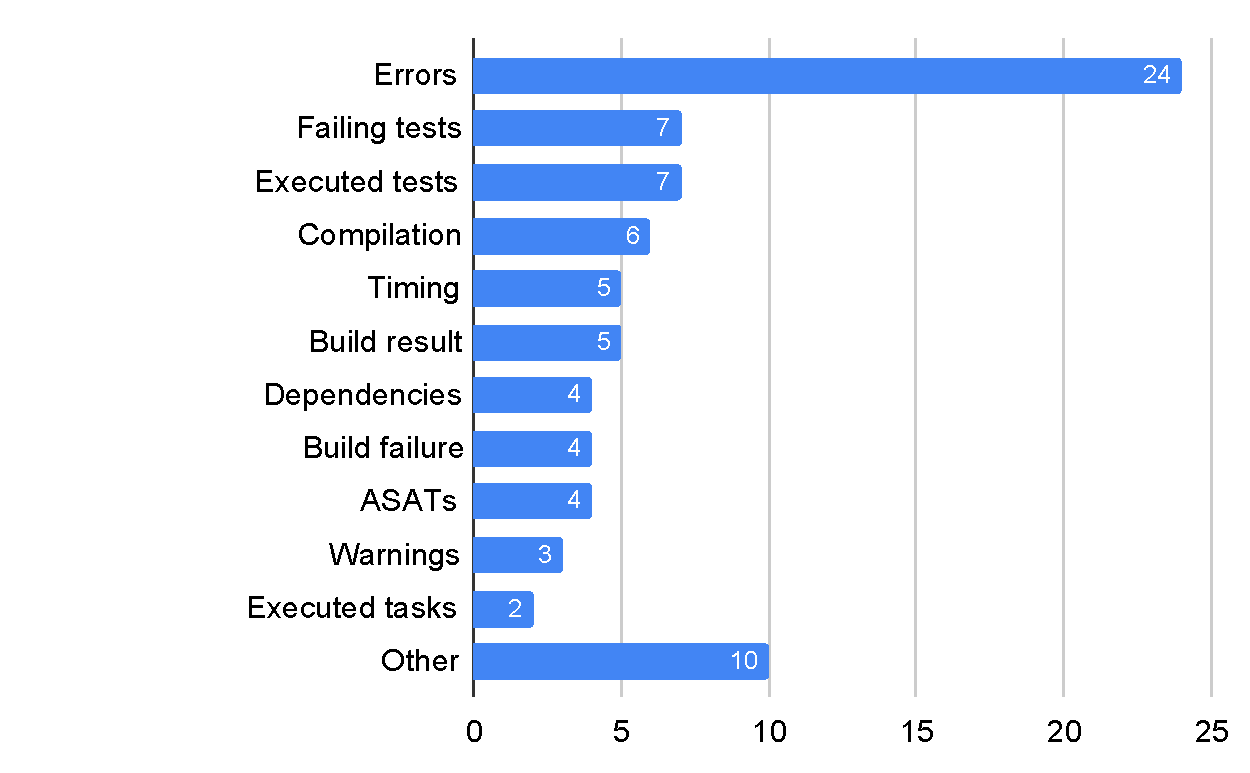
\includegraphics[width=\columnwidth,
		clip]{img/lit-sur/info_target.pdf}
		\caption{Information targeted in build log analysis.}
		\label{fig:litsur:info_target}

\end{subfigure}\hspace{\fill}
\begin{subfigure}[t]{\columnwidth}
		\centering
				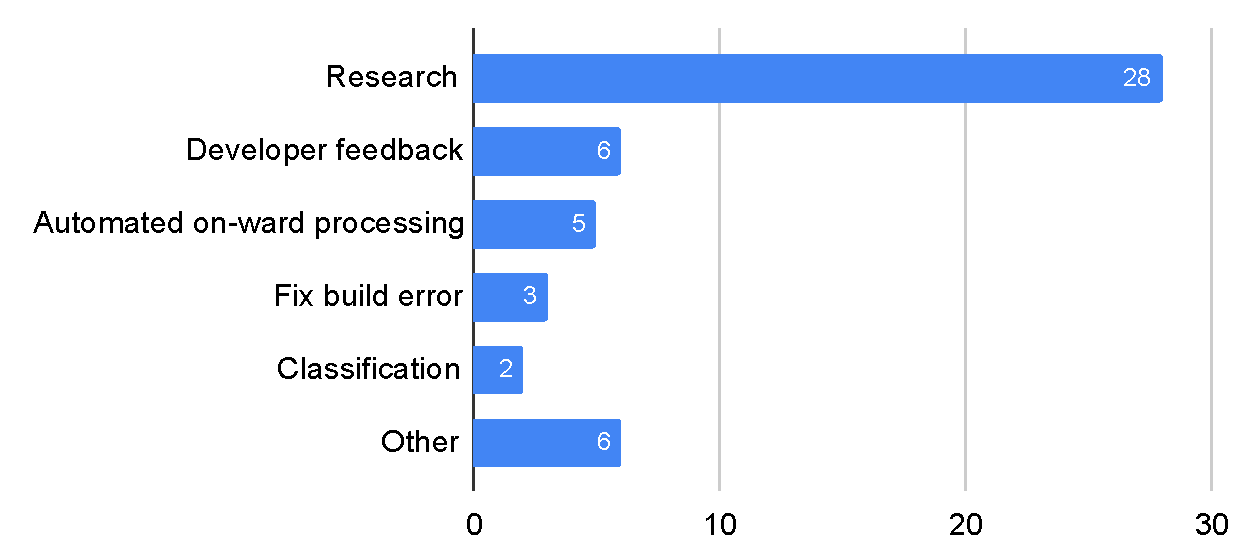
\includegraphics[width=\columnwidth,
				clip]{img/lit-sur/use.pdf}
		\caption{Purpose of build log analysis.}
		\label{fig:litsur:use}

\end{subfigure}

\caption{Multi-label categorization of the 61 relevant articles.}
\end{figure}

\subsection{Results}
In this section, we present the results of the analysis phase of the
literature mapping along RQ 1.1 through RQ 1.3.

% TODO repeat the question in the subsection title?
\subsubsection{Retrieved Information (RQ 1.1)}
% TODO General ref to Figure 4 missing: We answer this question along
% data in Figure 4, and ...
% ?

The precise information targeted in the build logs varied from article
to article.
\Cref{fig:litsur:info_target} gives an overview over the frequency of
the targeted information.
Most prominent was the search for errors (39\%), followed by extracting
the executed or the failing
tests (both 11\%).
There were also numerous works which targeted more specialized
information, such as the environments used during the
build~\cite{zolfagharinia2017not}, packages
installed~\cite{selberg2012use}, or hints to source files which
relate to build failures~\cite{ren2018automated}.

% TODO It is unclear where this comes from.
% TODO Also, wouldn't it perhaps be better to continue with Figure 4.b directly?
In most cases (51\%), a chunk was retrieved from the log.
Build logs were scanned for compilation
errors~\cite{clemencic2014new} or
the duration of tasks within the build~\cite{zhang2016android}.
36\% of the articles classified the build logs into categories.
For instance, distinguishing failures caused by developers from
failures caused
by infrastructure errors~\cite{lindqvist2019detection} or
whether projects use automated static analysis
tools~\cite{kavaler2019tool}.
Other types of information (e.g.,\ counting
lines, summarization) were only retrieved
in one case each.

The majority of articles (46\%) used the outcome of their build log
analysis for research purposes, as shown in \Cref{fig:litsur:use}.
% TOOD What does this mean? Give an example: to drive further research,
for example to categorize the types of compile errors encountered at
Google~\cite{}.
Further uses were giving feedback to developers (10\%) or automatic
on-ward processing of the retrieved information (8\%)
% TODO for example to ...
.

% TODO repeat the question in the subsection title?
\subsubsection{Retrieval Technique (RQ 1.2)}
\Cref{tab:litsur:techniques} presents the techniques that the articles
% TODO: lets use analyzing build logs canonically? Please search text
to eliminate occurrences of processing?
described for processing build logs.
% TODO This is weird.
Last number we have from above is 51.
43 of the 61 articles we inspected mentioned how they are analyzing build
logs.
However, only 16 of these described their method in detail.

The most mentioned method (34\%) was using a parser, where we also
included
rather imprecise statements like ``we parse the build logs.''
% TODO include citation?
% TOOD maybe make the point here that it is questionable whether this
includes a comprehensive tokenizer, lexer etc.
based solution and that parsing in many cases really meant regexp.
If we could figure that out, then we would assign it to regexp instead.
25\% of the articles described the use of regular expressions and 20\%
inspected the logs manually.
Another 8\% employed machine learning such as natural language
processing or information retrieval techniques.
For example,
Seo et al.~\cite{seo2014programmers} developed a custom
parser to classify error messages, while Vassallo et
al.~\cite{vassallo2017a-tale} analyzed build logs with regular
expressions.
Ghaleb et al.~\cite{ghaleb2019studying} used a compound approach.
They started with manual categorizing build logs and selecting
search strings that identify the target category.
Based on the search strings they created a script that automatically
classifies the remaining logs.

Only 25\% of the articles claimed their implementation is available.
Moreover, we
saw some reuse of the few available build log analysis tools.
Five articles employed the tools used to create
\emph{TravisTorrent}~\cite{beller2017travistorrent,beller2017oops,
orellana2017differences,zhao2018comparing} or
an extended version of them~\cite{rott2019empirische,
shi2018evaluating} (based on regular expressions),
two used the
\emph{Maven Log Analyzer}~\cite{macho2018automatically,gallaba2018noise}
% TODO: based on which technique?,
another two the
\emph{MAKAO}~\cite{wen2018blimp,adams2007design,adams2007makao} tool
% TODO: based on which technique?
.

\subsubsection{Build Logs}
% TODO using passive where it is unneccessary
The distribution of supported build tools is shown in
\Cref{fig:litsur:log_producer}.
Of the articles we surveyed, 30\% analyzed build logs produced by
Maven~\cite{maven2019website}, 16\% analyzed logs produced by
Gradle~\cite{gradle2020website}
and 10\% analyzed logs produced by Ant~\cite{ant2020website}.

% TODO remove first part of this paragraph?
Sometimes this limitation to a specific build tool is motivated by
aspects separate from the build log analysis.
For example, Shi et al.~\cite{shi2018evaluating} focussed on Maven
build logs because they also chose the PIT tool to calculate coverage
and mutation score.
A larger amount of the articles within our survey, however, limit
themselves to few build tools because their log format varies and
therefore ``parsers must be specialized to each build and test
framework''~\cite{tomassi2019bugswarm}.

Only 7\% of the proposed methods claimed to be language-agnostic, while
several described they are covering multiple source build tools.
The majority of articles (42\%) targeted logs from a source that no
second article
targeted.

% TODO death by passive
The main platform that build logs were collected from is Travis
CI~\cite{travisci2019webpage},
which was used in 38\% cases.
18\% of the articles processed logs from TravisTorrent and 8\% included
build logs from industrial projects.

% TODO perhaps remove this paragraph?
The number of logs analyzed varied greatly and we were not always able to
extract it confidently.
Articles reported processing from two up to 122 million logs.

31\% of the surveyed articles claimed to have published their data to
enable further research.
However, we found no clear reuse of build log data sets with the
exception of TravisTorrent~\cite{beller2017travistorrent}, which
Vassallo et al.~\cite{vassallo2017a-tale},
Ghaleb et al.~\cite{ghaleb2019studying}, and several other studies reused.

% TODO A and B should possibly be overlapping, otherwise there is an
% area where neither A nor B makes sense?
\begin{figure}[tbhp]
		\centering
		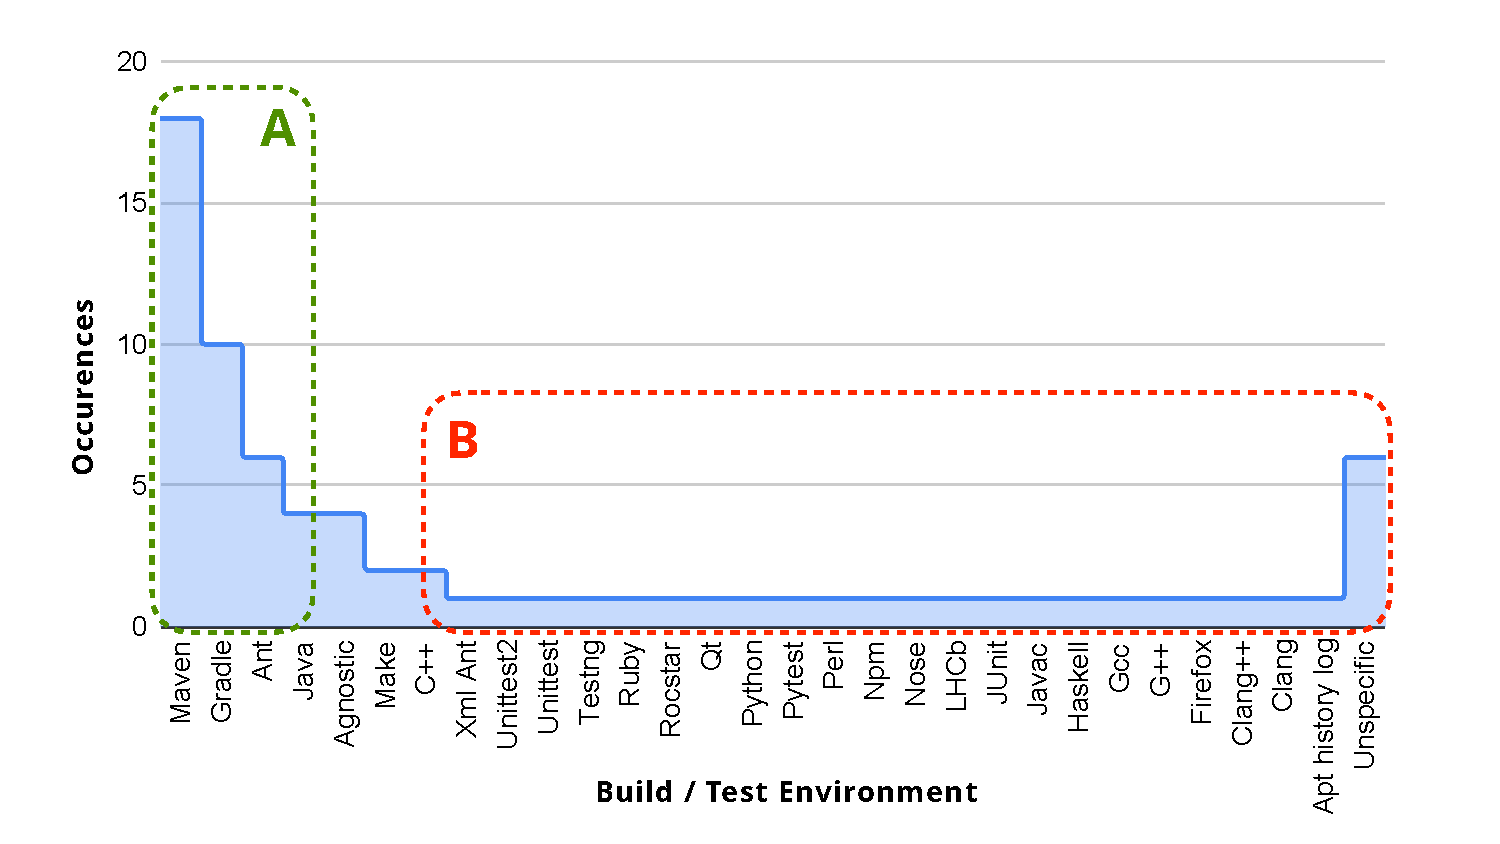
\includegraphics[width=\columnwidth, trim={1.1cm 0.4cm
		1.5cm 0.5cm},
		clip]{img/lit-sur/log_producer_annotated.pdf}
		\caption{Frequency of supported log producers.}
		\label{fig:litsur:log_producer}
\end{figure}


\subsection{Discussion}
\label{sec:lit-sur:discussion}
% TODO we are extracting failures in the following studies, which is mainly what
% literature does, too, right? Highlight here and mention later again

% TODO: this section is crucial.
% maybe we can highlight important findings, by categorizing them either
% as further subsubsections or making it bold in the text?
% TODO: find values for X and Y
Our literature survey shows that despite its relatively young age
(first occurrence of a paper on the topic in 2001, vast majority after
2016), \textbf{build log analysis is a widely established technique}
in the literature, with Y articles on it.


% TODO: this reads very hands-off and researchy.
% I don't understand the first sentence and would simply cut it.
We saw that various researchers process build logs, often because the
logs  provide more or the necessary
information to the researchers~\cite{ren2018automated}.
\textbf{Most log analysis is automated.} Automated approaches are
necessary as many studies target a large
number of builds.
Articles
which explicitly mention a manual analysis of the logs, mostly
restrict their work to few logs or take a ``representative sample to
make manual analysis feasible''~\cite{zolfagharinia2017not}.
% The chunk retrieval techniques we investigate within this article are
% automated, apart from their configuration through training examples.

% TODO: draw a conclusion together with figure 5: if reuse were higher,
lots of effort could be saved?
% discussion about popularity of replication packages adds nothing to
this paper.
We observed very little reuse of build log analysis tools.
This can stem from the fact that publishing replication packages and
research prototypes became popular only in recent years or from the
high specialization of the developed tools in regards to supported
build environments and targeted information.

Several articles noted the variety in log formats for different build
environments, which requires customizing build log techniques for
every supported build environment.
\Cref{fig:litsur:log_producer} shows that many studies and tools target
only a few distinct build environments (roughly, area A).
% TODO: passive ...
The majority of build environments was however only targeted by one
article each (B).
From this, we follow: (a) there is a nichè for custom parsers or even
specialized plugins integrated into the build process to make post-factum
parsing of logs redundant.
Plugins  similar to, for example, the Maven plugin to report test
executions Bell et al.
wrote, still have the disadvantage of not being able to work on historic
builds.
(b) the large tail of seldomly-investigated environments would benefit
from the existance of a more generic
solution.
% We implement build environment agnostic build log analysis
% techniques, which are customized to a specific project by
% the training examples which the user provides.
% In addition, the \emph{LogChunks}~\cite{brandt2020logchunks}
% data set we chose for our evaluation covers a broad range of build
% environments.
% % Further, the training examples also specify the log chunk targeted
% by the
% % retrieval, which enable our chunk retrieval techniques to retrieve
% % a broad range of information from build logs.

% TODO this is disconnected, at least here
Urli et al.~\cite{urli2018design} strongly discouraged from parsing
build logs for information as it is ``too error prone,'' other
articles pointed to the effort of developing a custom tool.
Regular expressions are known to be tedious to
maintain~\cite{michael2019regexes}.

% This task of retrieving specific chunks of text from the
% build logs can be solved by the chunk retrieval techniques we compare
% in this article.
% Our results can support researchers in choosing a
% suitable technique for their data set of build logs and the chunks
% they want to retrieve.
% By relieving them from building custom parsers
% we enable them to cover a much wider range of languages and build
% tools in their studies.

In summary, the results of the literature study show the need for
build log
analysis techniques that are automated, build-environment agnostic
% TODO who is the user?
and can be configured by the user with little effort.
% We achieve this by developing three techniques for which the
% information to be retrieved is specified through examples or keywords.


% TODO: the following paragraphs have nothing to do with a discussion
of the literature survey results.
% what we need is some derivation of the three techniques 1) regex 2)
cts 3) kws, best repeated here in the discussion and then from the lit
survey above, section 2.4.2
For this reason, we are focussing on techniques that run automatically
after being configured through examples or keywords.
Examples consist of logs and corresponding chunks.
The examples and keywords are provided by the user and can simply be
exchanged whenever new cases are introduced.

We propose the notion of chunk retrieval techniques which retrieve
a substring, that describes a specific information, from a build log.
Generally, these can also be used to classify build logs and therefore
cover the great majority of the type of log analysis we saw within
our survey.

We implement three chunk retrieval techniques based on approaches
described by several articles:
PBE mimics regular expressions and parsers while simplifying
their development.
We chose text similarity (CTS) as a common information retrieval
technique, and implement the ad-hoc approach of
searching for specific strings or keywords within KWS\@.

Our evaluation of the three chunk retrieval techniques is done on the
\emph{LogChunks} data set because it encompasses a broad range of
build environments which enables us to measure the generic
applicability of our techniques.
The targeted chunks are describing error messages or
``the reason the build failed,'' which was also the information
most targeted by the articles in our survey.

% The articles within our study mainly tried to retrieve or classify
% errors or reasons for the build to fail from the logs.
% Therefore we chose the log chunk ``describing why the build failed''
% ~\cite{brandt2020logchunks} for our empirical comparison study
% of chunk retrieval techniques.
% The techniques we implement are in principle agnostic to the targeted
% log chunk, thus we believe our results can be generalized to other
% kinds of log chunks.

\section{Chunk Retrieval Techniques}
\label{sec:techniques}

\begin{table*}[htb]
\centering
\caption{Chunk retrieval techniques.}
\begin{tabularx}{\textwidth}{@{}llXll@{}}
\toprule
Name			     & Acronym & Identification Technique
& Granularity & Configuration \\
\midrule
Program Synthesis by Example & PBE     & Regular expression program
& Character   & In/output examples	\\
Common Text Similarity	     & CTS     & TF-IDF \& cosine similarity,
expected number of lines & Line        & Output examples	   \\
Keyword Search		     & KWS     & Keywords, expected number of
lines			 & Line        & Keywords, context length  \\
Random Line Retrieval	     & RLR     & Random sample
& Line	      & Retrieval length	  \\
\bottomrule
\end{tabularx}
\label{tab:ctr}
\end{table*}

This section introduces key concepts of the three chunk retrieval
techniques we study in this article, namely program synthesis by
example (PBE), common text similarity (CTS), and keyword search (KWS).
In addition, we present our comparison baseline of random line
retrieval (RLR), illustrate the techniques on a concrete example
of log chunks and sketch out implementation.

% TODO this is not enough for Table 3. Where does it come from?
% How did it originate? Also: never single sentence abstracts
\Cref{tab:ctr} shows a comparison of the implemented techniques.

% TODO Somehow, we have to find a better place for this. We have been
% using the term 'chunk retrieval' beforehand already -- this
% definition now comes to late. The first paragraph should already
% apply to the literature mapping, the second of course only applies
% here.

\subsection{Characteristics of Chunk Retrieval Techniques}
\label{sec:crt-characteristics}
In this article, we evaluate different techniques to automatically
retrieve pieces of information that appear literally in the build
logs.
%, i.e., techniques that do not aggregate, combine, or deducted
%information.
We call such pieces of information from build logs
\emph{chunks}, and the techniques \emph{chunk retrieval techniques}.
The techniques we investigate here do not require a formal lexer and
parser to analyze the entire structure of build logs, but focus on
ad-hoc extracting just one specific piece of information per
configuration.

With the term \textit{configuration}, we abstract over the training
and parametrization that different techniques require in different
forms.
A configuration can be explicitly stated or implicitly derived
by learning through provided examples.
It is therefore a manual
specification of which information the chunk retrieval should target.
It also supplies the necessary information for the technique to
identify the targeted information chunk in a build log.
Each chunk
retrieval technique has a specific \textit{granularity}, i.e.,\ the
smallest piece of text it can return (e.g., a line, or a word).
The
granularity might be adjustable by configuration.
\emph{Running a
chunk retrieval technique} means executing a fully configured
technique to consumes as input a build log in plain text format and to
produce an array as output.
The array consists of substrings of the
build log text.

\subsection{Program Synthesis by Example (PBE)}
The concept of \emph{Programming by Example} aims to capture the
intent of the user through examples which they provide.
Leveraging this approach, we implemented a chunk retrieval technique
for build logs.
Our implementation is based on the
\emph{PROSE library}~\cite{prose2019webpage}.
The PROSE library is powered by the generic program synthesis framework
\emph{FlashMeta}~\cite{polozov2015flashmeta:} and the specialized
text extraction DSL \emph{FlashExtract}~\cite{le2014flashextract:}.
Both enable us to synthesize regular expression programs
consistent~\cite{mitchell1982generalization} with a set of in-
and output examples given by the user.
The usage of example enables the user to configure a chunk
retrieval without understanding the whole structure of
the build log.

\subsubsection{Configuration}
In- and output example pairs are the main driver of Programming by
Example; we refer to them in short as \emph{examples}.
The \emph{input} is the text of the build log file.
The \emph{output} is
a substring of the log file text, representing the
substring that should be retrieved by the synthesized program when
given the corresponding input file.
One or multiple examples, the
training set, \emph{configure} a specific chunk retrieval with PBE:
they define the substring of a build log that should be extracted.
The PROSE program synthesis then tries to construct a program
consistent with all training examples.
If PROSE cannot synthesize a program, e.g.,\
because the regular expression
necessary would be too complicated to synthesize, PBE returns the
error message ``no program found.''
% TODO Figure 7 should not come before Figure 6. Figure 6 and 7 should be
% introduced first. This is best-practice anyway: Whenever you mention
% a figure/table the standard sentence should always be: Figure X shows Y,
% on the vertical axis Z and on the horizontal axis D.

\Cref{lst:prose-program-simplified} presents a simplified version
of a program learned from the examples in \Cref{lst:chunk-example}.

% TODO Moritz: you said: The following is very obvious and could apply
% to any
% % technique.
% % kinda.
% It does give a descriptive error message on no match (and
% % that is not possible in other techniques)
% % otherwise yes, nothing interesting happens in the application of pbe
% % though for consistency we might need this section? or merge
% config/application?
% TODO Why does it return an error message? Shouldn't it also return
% <empty string>? Does it not rather return an error message if no
% program can be synthesized?
\subsubsection{Application}
A run of PBE takes a build log file as input and applies the
synthesized regular expression program.
It then returns the substring
of the build log matched by the program or an error message if the
program found no match. 


\subsection{Common Text Similarity (CTS)}
Text Similarity approaches are widely used to filter unstructured
textual software artifacts~\cite{runeson2007detection,
marcus2005recovery,antoniol2002recovering,mccarey2006recommending}.
We investigate a chunk retrieval technique based on the common
% TODO: the ominuous Vector Space Model again ...
Vector Space Model~\cite{schutze2008introduction}.
The aim is to retrieve those lines from a build log which are most
similar to examples given by the user.

\subsubsection{Configuration}
To configure chunk retrieval through text similarity we chose to use
the same concept of examples as for PBE
% TODO Moritz: your question was: More details on this.
% How do you
% 'apply' VSM? On what?
% all the following sentences in this subsubsection describe our way
% of determining text similarity which as far as I understand and
% Annibale said is the VSM.
% word tokens, tf-idf, similarity measure
% I added a "as follows", think that is enough for explanation?
% TODO: I think it is good, but the VSM is still unexplained. We need a
% (at least) 1-sentence introduction to it, at its first reference
and apply the Vector Space Model~\cite{schutze2008introduction}
as follows:
The lines of the output strings of the training examples define our
search query.
The algorithm splits the search query into single lines and
identifies tokens, in our case words.
Then we build a
document-term-frequency matrix over the lines from the search query
and prune very often or very rarely appearing words.
Finally, the
algorithm applies TF-IDF to the matrix, a best practice for natural
language queries~\cite{lee1997document}.

\subsubsection{Application}
To retrieve the desired information from a build log, we parse the
whole text and process it in the same way as the search query.
The algorithm calculates the cosine
similarity~\cite{korenius2007principal} to compare each line of the
build log with each line of the search query.
After summing up the
similarities of each build log line to all search query lines, we sort
the build log lines in decreasing similarity.
The average number of
lines in the outputs of the training examples determines how many of
the most similar lines are returned as the output of the retrieval
run.

\subsection{Keyword Search (KWS)}
When developers scavenge for a specific piece of information within a
large amount of unstructured information, a first ad-hoc approach they
use is to search for related keywords.
Indeed, this was one of the
most common approaches we took when searching for the reason a build
failed while creating the \emph{LogChunks} data
set~\cite{brandt2020logchunks}.

\subsubsection{Configuration}
A set of keywords configures the chunk retrieval with KWS\@.
To better
compare KWS with PBE and CTS, we also configure it through examples.
We associate each example with keywords which appear in the targeted
chunk or close to it.

KWS then searches for those keywords which are tied to the greatest
number of examples in the training set.
If several keywords are associated with the same number of training
examples, and no other keywords are associated with more training
examples, KWS searches for all of these keywords.

\subsubsection{Application}
For a retrieval run, we take a whole build log file as input and
search for all exact occurrences of the keywords.
As keywords are
often not directly describing the desired information, but rather
appear close to the desired information, KWS also retrieves the lines
around the found keyword.
The number of surrounding lines retrieved is
the average of lines in the output of the training examples.


\subsection{Random Line Retrieval (RLR)}
\label{sec:expl-rlr}
% TODO: could you add two-three more references to the results of RLR in
% the discussion, to show how even seemingly low numbers are much better
% than RLR?

To fully comprehend how difficult a task build log analysis really is without any a-priori knowledge, we include a comparison with a base line generated by Random Line Retrieval (RLR), that is,
picking lines randomly from the build log.
RLR mimics the
situation of guessing blindly which lines might be interesting.
The only configuration option for RLR is the number of lines it should
retrieve.
For a fair comparison to the other techniques (whose number of
returned lines is dynamic), we configure RLR to return the average
number of lines in the chunks of the training examples, thus arguably giving it a slight advantage.

% TODO Moritz: you said: some more details here?
% I would not know of any details to add.
%It's really all we are doing
% TODO: You are right, nothing more is necessary


% TODO: these next two sections do not belong under this section -- they are not a chunk retrieval technique. One way to fix it would be to rename the section.
\subsection{Chunk Retrieval Example}
\label{sec:crt-example}

\begin{figure}[tbp]
  \centering
\begin{subfigure}[tbp]{\columnwidth}
  \begin{lstlisting}[breaklines=true,frame=tlr]
FAILURE: Build failed with an exception.

* What went wrong:
  \end{lstlisting}
  \vspace{-\baselineskip}
  \begin{lstlisting}[backgroundcolor=\color{Cerulean!60},breaklines=true,frame=rl]
Could not determine the dependencies of task ':app:jacocoTestDebugReport'.
> Task with path 'testDebug' not found in project ':app'.
  \end{lstlisting}
  \vspace{-\baselineskip}
  \begin{lstlisting}[breaklines=true,frame=blr]

* Try:
  \end{lstlisting}
\end{subfigure}\hspace{\fill}
\begin{subfigure}[tbp]{\columnwidth}
  \centering
  \begin{lstlisting}[breaklines=true,frame=tlr]
FAILURE: Build failed with an exception.

* What went wrong:
  \end{lstlisting}
  \vspace{-\baselineskip}
  \lstinputlisting[backgroundcolor=\color{Cerulean!60},breaklines=true,frame=rl]{listings/chunk1.txt}
  \vspace{-\baselineskip}
  \begin{lstlisting}[breaklines=true,frame=blr]

* Try:
  \end{lstlisting}
\end{subfigure}
  \caption{Two examples of log chunks explaining why an Android
  build failed.}
  % TODO Moritz: we can relate this to travistorrent maybe, you told me
  % long ago that this was something your analyzer cannot extract
  \label{lst:chunk-example}
\end{figure}

\lstset{language=caml, morekeywords={StartExtraction, RegexPosition,
RegexPair,
  EndExtraction}, keywordstyle=\bfseries\color{black}, escapeinside=//}
\begin{figure}[tbp]
  \centering
  \lstinputlisting[breaklines=true]{listings/prose.txt}
  \caption{Simplified regular expression produced by PBE when trained
  with examples from \Cref{lst:chunk-example}}
  \label{lst:prose-program-simplified}
\end{figure}

\lstset{
  language=,
  morekeywords={},
  texcl=false
}
\begin{figure}[tbp]
  \centering
  \begin{lstlisting}[breaklines=true,frame=tlr]
=== RUN   TestSeparator
  \end{lstlisting}
  \vspace{-\baselineskip}
  \lstinputlisting[backgroundcolor=\color{Cerulean!60},breaklines=true,frame=rl]{listings/chunk2.txt}
  \vspace{-\baselineskip}
  \begin{lstlisting}[breaklines=true,frame=blr]
=== RUN   TestGenerateHTML
  \end{lstlisting}
  \caption{Example of a log chunk showing a linter error}
  \label{lst:chunk-example-3}
\end{figure}

To illustrate the chunk retrieval techniques further, we want to give
an example of real-world log LogChunks.
\Cref{lst:chunk-example} shows two excerpts
from Android build logs.
Marked in blue are the chunks
which contain the information on why the
corresponding build failed.

When PBE is trained with these two examples, it produces
a regular expression program similar to the one presented in
\Cref{lst:prose-program-simplified}.
The retrieval
starts after a colon and a line separator and before a capital
letter.
It ends before two line separators,
which is consistent with the two example
chunks from \Cref{lst:chunk-example}.
This shows, that the characters structuring the text around the chunk are
crucial for regular expressions to identify a log chunk.
In fact, if the third example from \Cref{lst:chunk-example-3},
which has a
different structural representation, is added to the training set,
PBE is not able to synthesize a program and returns
``\texttt{no program found}.''
We later express this difference in structural representation through
dividing log chunks into \emph{structural categories}.
The chunks from \Cref{lst:chunk-example}
are in the \emph{same structural category}, while the chunk from
\Cref{lst:chunk-example-3} is in a
\emph{different structural category}.
The results of our empirical comparison study on the chunk retrieval
techniques
show that the structural representation of the targeted chunk greatly
influences
the performance of the chunk retrieval techniques.

CTS will rank the lines from an analyzed build log which are most
similar to the chunks in the training examples
from \Cref{lst:chunk-example}.
It will then return the two lines ranked highest, as the chunks in
the training examples have on average two lines.

KWS is configured with keywords that appear close to the chunk within
the build log.
For the examples from \Cref{lst:chunk-example} these could be
``FAILURE,'' ``wrong,'' or ``failed''.
The example from \Cref{lst:chunk-example-3} could be found
by searching for ``FAIL.''
If KWS was to be trained with all three examples and the aforementioned
associated keywords, it would search for the three keywords from
\Cref{lst:chunk-example}, as they appear twice---most often within
the training set of three examples.

\subsection{Tool Implementation}
For our comparison study, we implemented each of the chunk retrieval
techniques and a unifying interface.
The unified interface is implemented in Ruby and
calls the separate technique implementations over the command line.
We implemented PBE in C\# based on the Microsoft PROSE
library~\cite{prose2019webpage} and CTS, KWS, and RLR using
R and the text2vec library~\cite{text2vec2019webpage}.
% TODO and passive again ...
The source code of the implementation can be found in our replication
package~\cite{brandt2020chunk-replication} together
with ready-to-use Docker images.

\section{Study Design}

% TODO This section is not structured well. First, it misses an
% explanation of the bigger study design.  Second, What is the difference between Study Process and
% Study Design? Third, the LogChunks section appears out of nowhere
% and is not related to the section title (different abstraction
% level).  Perhaps a solution would be to be a bit inspired by this
% paper:
% https://inventitech.com/publications/2018_beller_spruit_spinellis_zaidman_on_the_dichotomy_of_debugging_behavior_among_programmers.pdf
% There is a research design section (which we are missing) and a
% Research Method section (which is a mixture of the current section
% titled Log Chunks and Study Process)

\label{sec:study}

To investigate when the chunk retrieval techniques are suited to
analyze build logs (\textbf{RQ2}), we perform an empirical comparison
study on the \emph{LogChunks} data set~\cite{brandt2020logchunks}.
In particular, we are interested in how many examples a technique
should be trained with (\textbf{RQ2.1}),
how similar the structural representation of the targeted log chunks
has to be (\textbf{RQ2.2}) and how reliable the quality of the
produced outputs is (\textbf{RQ2.3}). This leads us to the following research questions:

\begin{simplebox}[minipage boxed title*=-1.5cm,
attach boxed title to top center={yshift=-6mm}]
{\textbf{RQ2:} What are the comparative strengths and weaknesses
of promising build log analysis techniques?}
\begin{itemize}[leftmargin=1.2cm]
  \item[\textbf{RQ2.1:}] How many examples does a technique need to
  perform best?
  \item[\textbf{RQ2.2:}] How structurally similar do the examples
  need for a technique to be applicable?
  \item[\textbf{RQ2.3:}] How accurate are the retrievals of a technique?
\end{itemize}
\end{simplebox}

In the following, we present the data set we created for this study,
our study process (presented in \Cref{fig:study}) and the metrics
we measure to answer our research questions.

\begin{figure*}[tb]
	\centering
	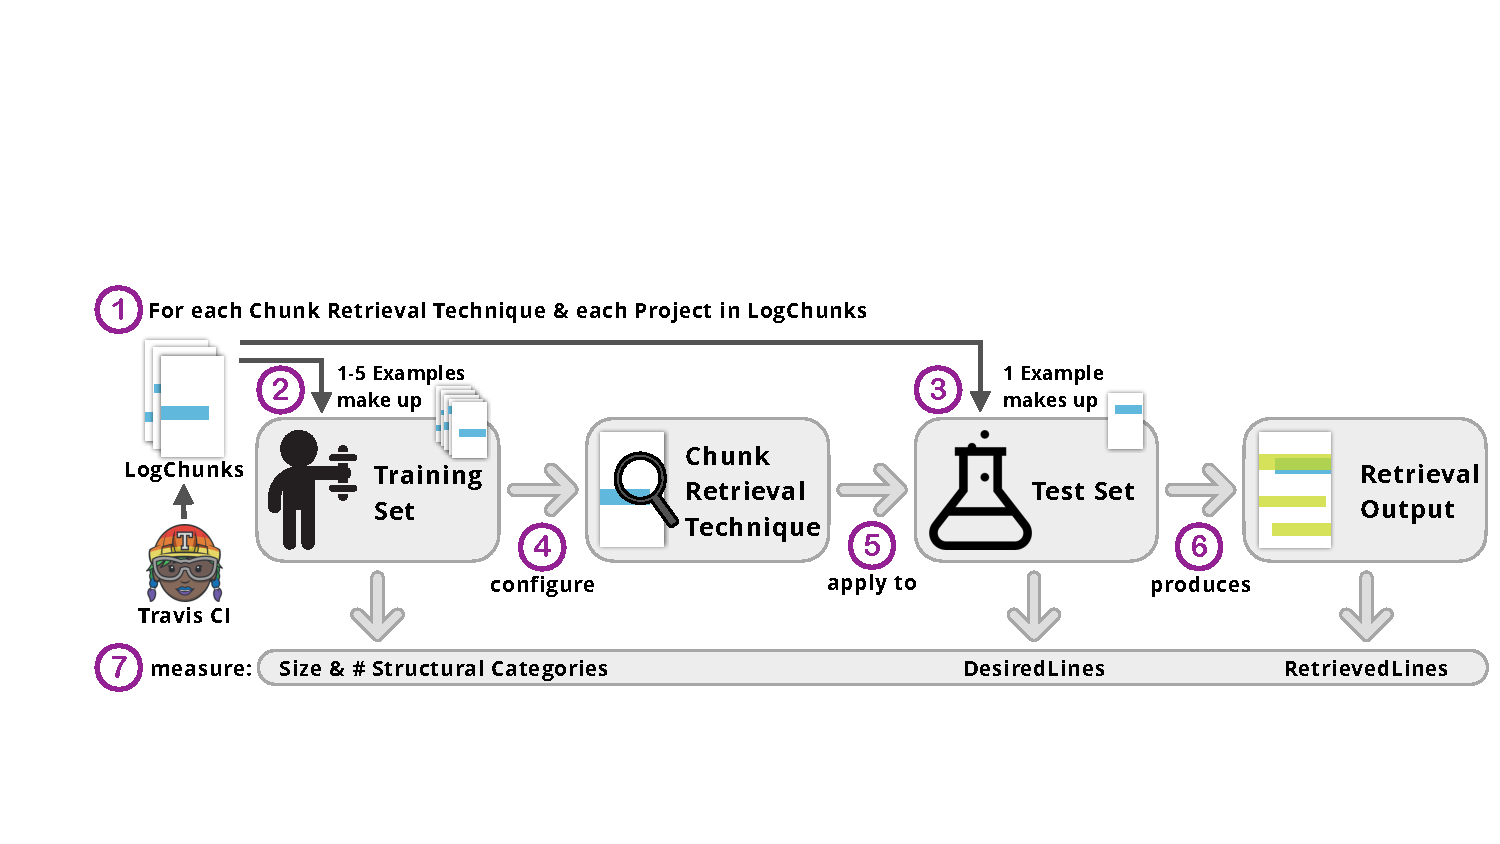
\includegraphics[width=\textwidth, trim={1.6cm 1.6cm 0.2cm 5.6cm},
  clip]{img/study.pdf}
	\caption{Design of our technique comparison study.}
	\label{fig:study}
\end{figure*}


\subsection{LogChunks}
To conduct the study in this paper, we created the 
\emph{LogChunks}  data set~\cite{brandt2020logchunks}.
It encompasses 797 build logs from Travis CI,
stemming from a broad range of 80 GitHub repositories and 29
programming languages.
For each file, the authors manually ``labeled
the log part (chunk) describing why the build
failed''.
We included keywords, which we
would use to search for the selected chunk within the log.
In
addition, we categorized the log chunks according to their format
within the log.
If the chunks were surrounded by the same markings
within the log, we assigned them the \emph{same structural category},
as described in \Cref{sec:crt-example}.

\subsection{Study Process}
% TODO: I think you need to introduce a concept that makes clear what one
% ``folder'' consists of ...
% TODO: What does this mean -- we begin by? Aren't we perhaps missing that
% we operate on all repos in LogChunks?
We begin by selecting all examples in \emph{LogChunks}
that correspond to one GitHub repository---and thus the
% TODO () is meant to reference the figure, but this the figure is not actually mentioned.
same build environment (1).
% TODO: What does this mean? Of what nature are the examples? How were they chosen?
% Isn't it rather the case that for each repository, we built traning sets of size 1, 2,
% ... 5 build logs?
One to five examples make up the training set (2).
% TODO passive ...
We vary its size to measure how many examples are needed to
confidently configure a technique.
The training set is so small because the examples have to be
manually created by a user.
A larger training set would oppose our goal of providing techniques
that can be configured with little effort
(see \Cref{sec:lit-sur:discussion}).
% TODO: The example? why only one? And what is an example? An example build log?
% Then it would be good to say so.
The example chronologically after the training set makes up the
test set (3).
In this way, we train on examples from past build logs and test on
more recent logs.
We chose a test set size of 1, as users of our techniques
should receive reliable results on every build log they analyze.
% TODO and why is this important? Doesn't everyone want such stability of results?
In the next step, we configure a chunk retrieval technique with
the examples from the training set (4) and apply the technique to the
training set (5), which produces the retrieval output (6).
Based on this, we collect the following measurements (7):
the size of the training set (\textbf{RQ2.1}),
the number of structural categories in the training
set (\textbf{RQ2.2}),
the lines of the retrieval output ($\mathit{RetrievedLines}$),
and our oracle: the output defined in the test example
($\mathit{DesiredLines}$).
From these we calculate accuracy metrics (\textbf{RQ2.3}):

\vspace{0.2cm}
\begin{itemize}[leftmargin=0.4cm] \itemsep1em
	\item $|\mbox{True\ Positives}| = \mathit{DesiredLines} \cap
	\mathit{RetrievedLines}$ \vspace{0.2cm}\\
	True positives are lines that appear both in the output of a
	tool as well as what \textit{LogChunks} contains for the
  test example.

	% What about when a line is replicated twice?
	% I.e., Are line numbers part of this? => no.
	% not checked, but if lines are identical they also contain
	% the same information so if someone asks we can defend I think

	\item $\mbox{Precision} = \dfrac{|\mathit{True\
	Positives}|}{|\mathit{RetrievedLines}|}$ \vspace{0.21cm} \\
	Precision of a chunk retrieval describes which proportion of
	the retrieved lines were actually desired.

	\item $\mbox{Recall} =
	\dfrac{|\mathit{True\ Positives}|}{|\mathit{DesiredLines}|}$
	\vspace{0.2cm} \\
	Recall of a chunk retrieval describes which proportion of the
	desired lines were retrieved.

	\item $\mbox{F$_{1}$-score} = 2 \cdot \dfrac{\mathit{Precision}
	\cdot \mathit{Recall}}{\mathit{Precision} + \mathit{Recall}}$
	\vspace{0.2cm}\\
	In addition, we calculate the F$_{1}$-score, the harmonic mean
	of precision and recall.
  We prefer F$_{1}$ to other aggregate
	measures such as accuracy because for a
	``needle-in-the-haystack'' scenario, we want to avoid bloating
	our results by correctly not finding lots of irrelevant log
	lines.

	\item Successful retrieval = $\mathit{true}\ \mathit{iff}\
	\mathit{Recall} = 1, \mathit{false\ otherwise}\vspace{0.1cm}$

	We define a successful retrieval as one where all desired
	lines were
	extracted, therefore when recall is one.
\end{itemize}

% This is a weird position for this paragraph
% TODO What is ``this'' referring to? You just defined a bunch of equations.
This concludes one execution within our evaluation.
% TODO run vs. execution above.
We conduct one run for each of the four chunk retrieval techniques,
for each of the eighty repositories in \emph{LogChunks} (8)
and for each of the five training set sizes (2).
In total we perform 1600 runs, 400 for each of the implemented chunk retrieval
technique.

\section{Results}
This section first presents the results for each chunk retrieval
technique separately.
Afterwards, we compare the three techniques with each other and to RLR as a
baseline.



\subsection{Program Synthesis by Example (PBE)}
\label{sec:r:pbe}

\begin{figure}[tbp]
		\centering
		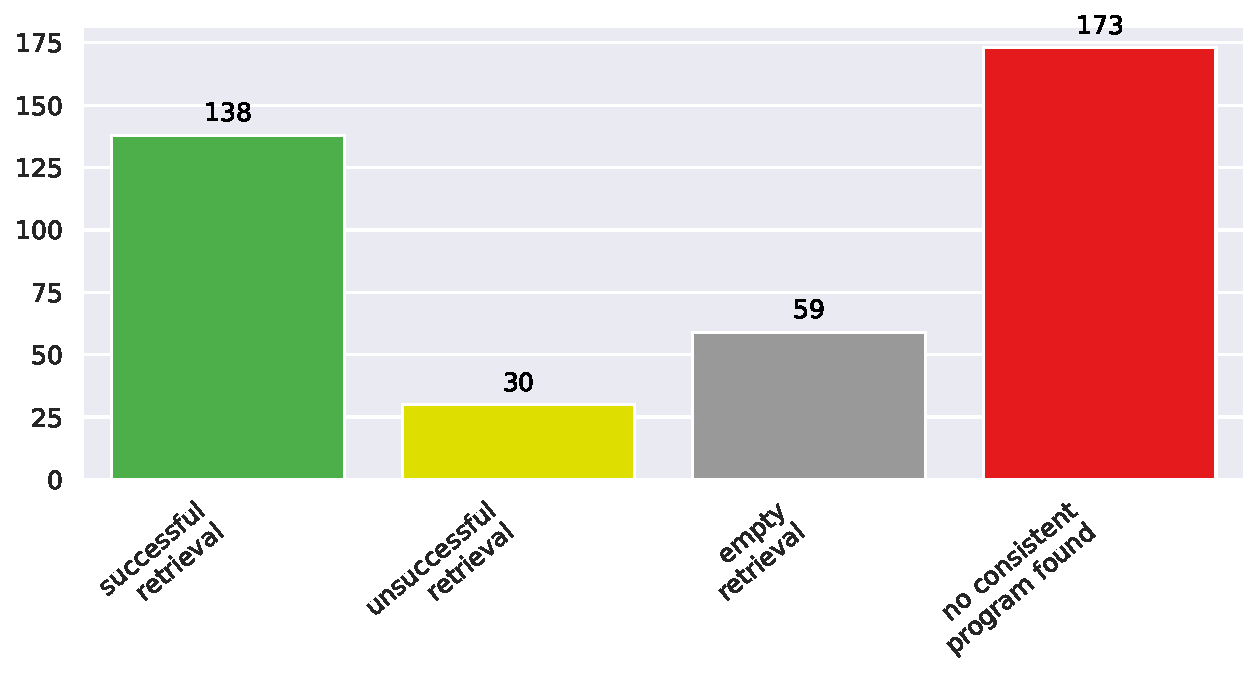
\includegraphics[width=\columnwidth,
		clip]{img/big-study/failure-reason-pbe.pdf}
		\caption{Results of chunk retrieval with PBE.}
		\label{fig:failure-reason-PBE}
\end{figure}

\lstset{
  language=,
  morekeywords={Test, Output, Desired},
  keywordstyle=\textbf,
	frame=single
}
\begin{figure}[!t]
  \centering
  \begin{lstlisting}[breaklines=true]
Test Output:
Error: Invalid CSS after "2.3em": expected expression (e.g.
1px, bold), was ";"
	on line 86 of sass/components/dropdown.sass
Desired Test Output:
Error: Invalid CSS after "2.3em": expected expression (e.g.
1px, bold), was ";"
	on line 86 of sass/components/dropdown.sass
	from line 5 of sass/components/_all.sass
	from line 6 of bulma.sass
  \end{lstlisting}
  \caption{Example for an unsuccessful retrieval (PBE retrieved only
  two of the four targeted lines).}
  \label{lst:pbe-unsuccessful}
\end{figure}

\begin{figure*}
\centering
    \textbf{Program Synthesis by Example (PBE)}\par\medskip
\begin{subfigure}[b]{\columnwidth}
		\centering
		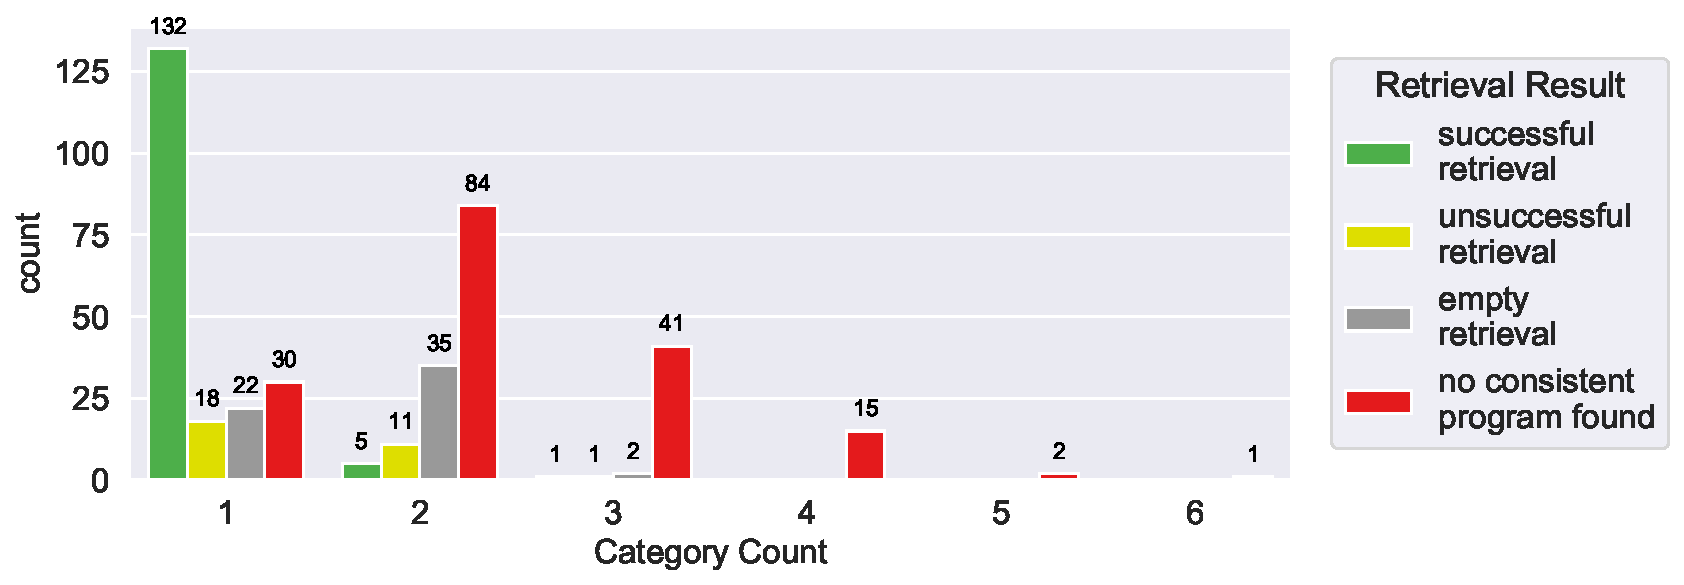
\includegraphics[width=\columnwidth,
		clip]{img/big-study/failure-reason-categorycount-PBE.pdf}
				\caption{Successfulness of retrieval
				compared by structural category count
				in training and test sets.}
		\label{fig:failure-reason-categorycount-PBE}
\end{subfigure}\hspace{\fill}
\begin{subfigure}[b]{\columnwidth}
		\centering
		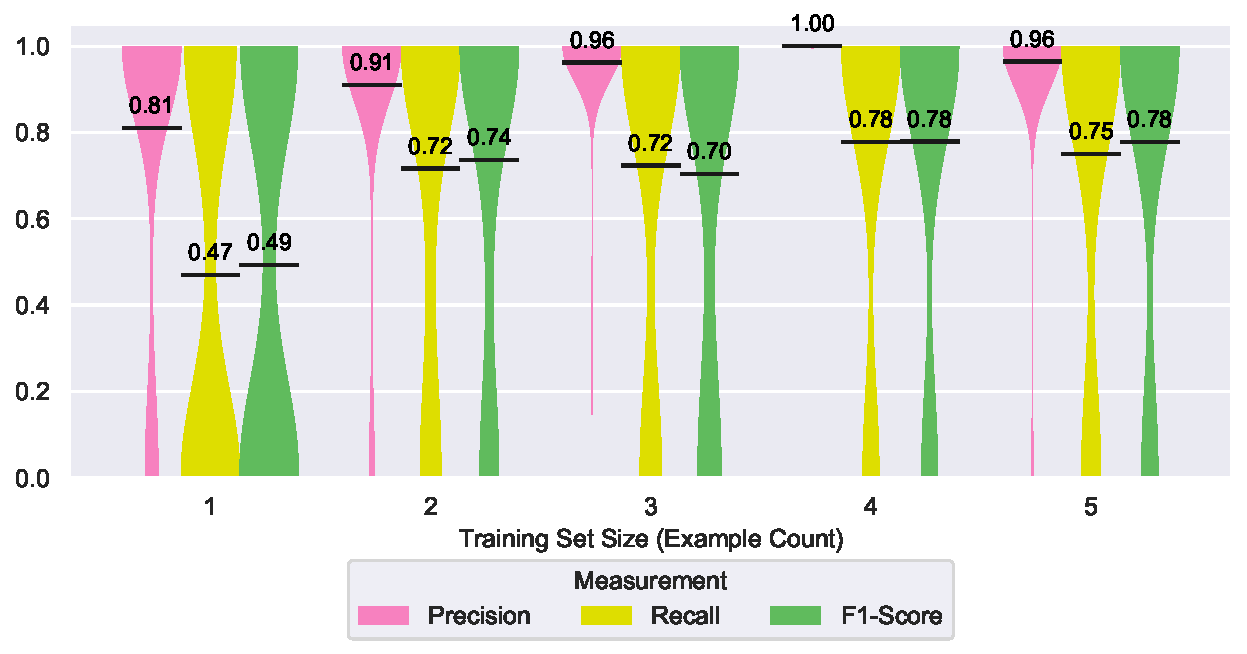
\includegraphics[width=\columnwidth,
		clip]{img/big-study/recall-precision-examplecount-sythesisworked-PBE.pdf}
				\caption{Precision, recall and
				F$_{1}$-score when PBE could synthesize
				a consistent program compared with the
				size of the training set.}
		\label{fig:recall-precision-examplecount-sythesisworked-PBE}
\end{subfigure}
\caption{Results of chunk retrieval with  Program Synthesis by Example
(PBE)}
\end{figure*}

% TODO Say something about this being a pecularity of PBE ...
\Cref{fig:failure-reason-PBE} shows the results of chunk
retrieval with PBE.
Out of the overall 400 runs, 5 per each one of the 80 example
sets, PBE extracted all desired lines successfully in 138 cases.
In 59 cases, a regular expression program could be synthesized, though
it did not find match on the test build log.
In 30 cases, the synthesized program only extracted a
subset of the desired lines.
For these 30 cases, the average recall
was 28\%.
% TODO: Perhaps we should call it partially successful? Let's
% discuss this in a meeting
\Cref{lst:pbe-unsuccessful} shows how an example of such
an \emph{unsuccessful retrieval} looks like. In it, the synthesized program only
retrieved two of the four targeted lines.
In 173 of the 400 cases
could PROSE not synthesize a program consistent with all of the training
examples.

% TODO introudce this fig at large. Soemthing like: Zooming in
% on only the successful retrievals from (...), Fig ... shows ...

\Cref{fig:failure-reason-categorycount-PBE} shows the results of PBE
runs depend on the number of structural categories in the training and
test examples.
The figure demonstrates that program synthesis mostly
returns exactly the desired output when there are is only one
structural category present in the training and test examples.
However, when
two or more structural categories are simultaneously present,
PROSE could in most cases not synthesize a program.
For four or more present
categories PROSE could never synthesize a consistent program.

\Cref{fig:recall-precision-examplecount-sythesisworked-PBE} shows
precision and recall of the 227 runs where PBE could synthesize a
program consistent with all training examples.
When the training set
size increases from one to two, recall and F$_{1}$-score increase by
about 25\%, precision increases by about 10\%.
For two or more
training examples, recall and F$_{1}$-score stay around 75\% and
precision around 96\%.

\subsection{Common Text Similarity (CTS)}
\label{sec:r:cts}
\begin{figure*}
\centering
    \textbf{Common Text Similarity (CTS)}\par\medskip
\begin{subfigure}[tb]{\columnwidth}
		\centering
		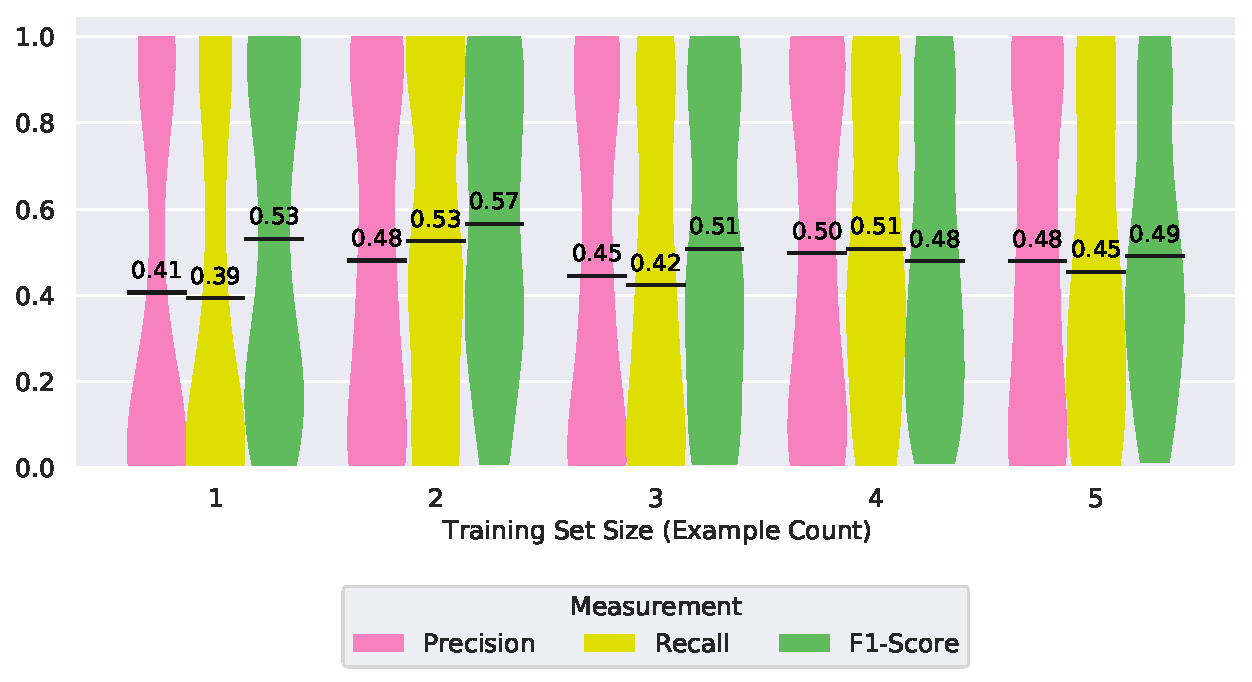
\includegraphics[width=\columnwidth,
		clip]{img/big-study/recall-precision-examplecount-CTS.pdf}
		\caption{training set size.}
		\label{fig:recall-precision-examplecount-CTS}

\end{subfigure}\hspace{\fill}
\begin{subfigure}[tb]{\columnwidth}
		\centering
				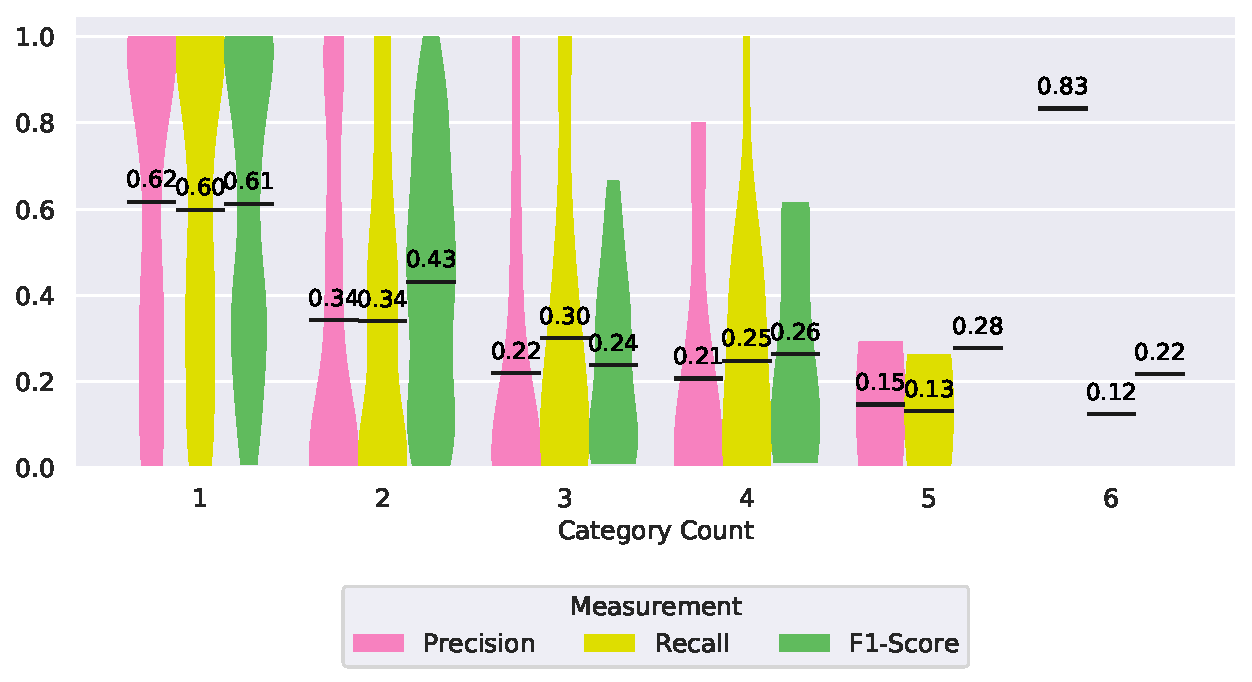
\includegraphics[width=\columnwidth,
				clip]{img/big-study/recall-precision-categorycount-CTS.pdf}
		\caption{structural category count
		in training and test set.}
		\label{fig:recall-precision-categorycount-CTS}
\end{subfigure}
\caption{Precision, recall and F$_{1}$-score of chunk
retrieval with Common Text Similarity (CTS) compared by \ldots}
\end{figure*}

% TODO what about referencing the combined figure at first: something like shows the results of CTS on two beanplots of ... and ...., and then the subfigure
% TODO this goes for all techniques
\Cref{fig:recall-precision-examplecount-CTS} presents precision,
recall and F$_{1}$-score of chunk retrieval using CTS for an
increasing number of training examples.
When using one to five
training examples, the size of the training set has no noticeable
influence on precision, recall or F$_{1}$-score of the chunk retrieval
with CTS.

\Cref{fig:recall-precision-categorycount-CTS} shows the same
measurements for an increasing number of structural categories in the
training and test examples.
With increasing category count, precision,
recall and F$_{1}$-score decrease.
% Especially for more than four
% categories present we have no chunk retrieval runs where all desired
% lines were extracted.

\subsection{Keyword Search (KWS)}
\label{sec:r:kws}
\begin{figure*}
\centering
    \textbf{Keyword Search (KWS)}\par\medskip
\begin{subfigure}[b]{\columnwidth}
		\centering
		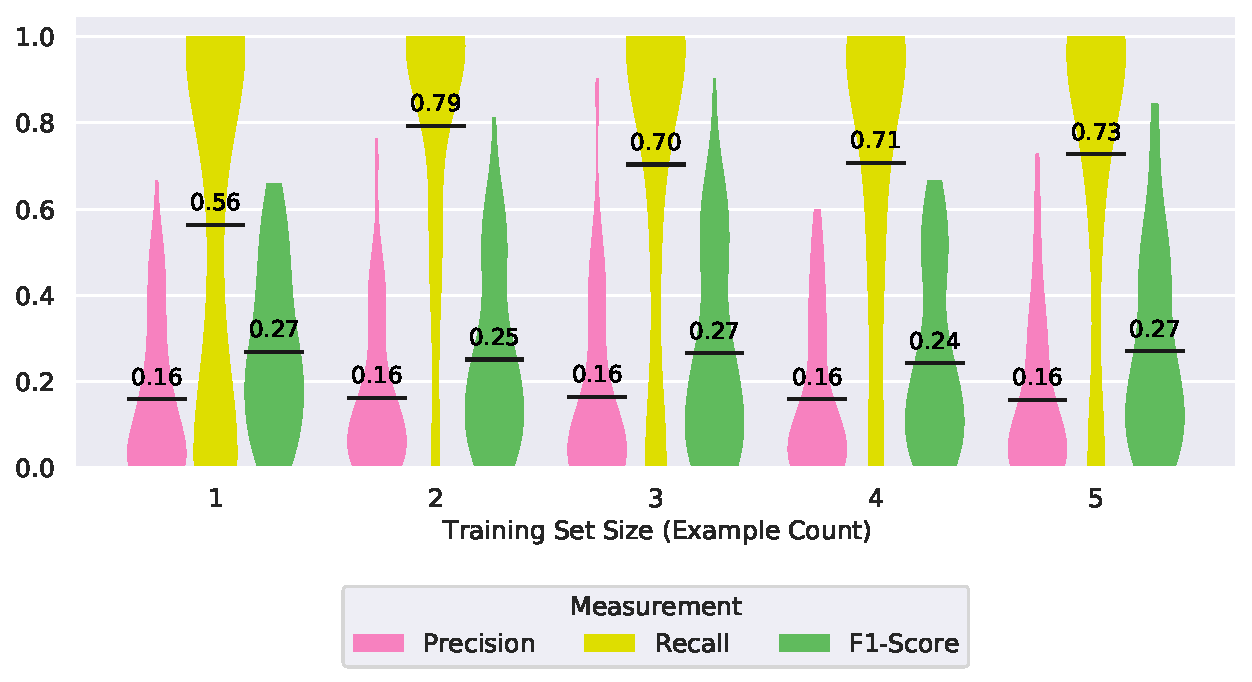
\includegraphics[width=\columnwidth,
		clip]{img/big-study/recall-precision-examplecount-KWS.pdf}
		\caption{training set size.}
		\label{fig:recall-precision-examplecount-KWS}
\end{subfigure}\hspace{\fill}
\begin{subfigure}[b]{\columnwidth}
		\centering
		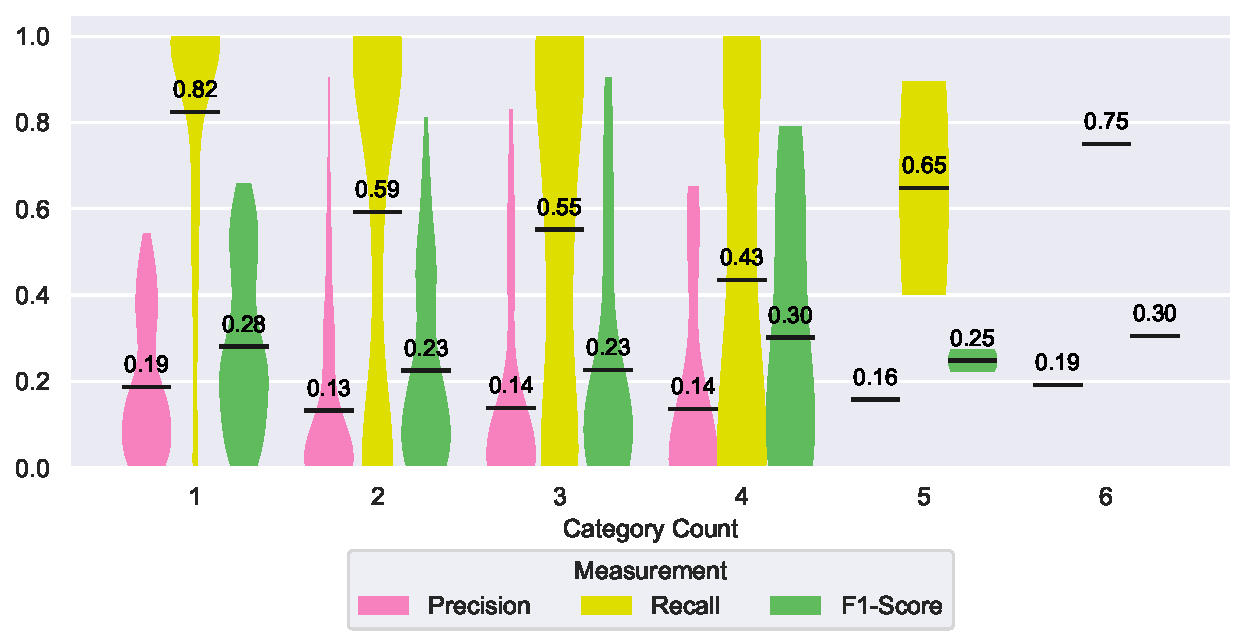
\includegraphics[width=\columnwidth,
		clip]{img/big-study/recall-precision-categorycount-KWS.pdf}
		\caption{structural category count
		in training and test sets.}
		\label{fig:recall-precision-categorycount-KWS}
\end{subfigure}
\caption{Precision, recall and F$_{1}$-score of chunk retrieval with
Keyword Search (KWS) compared by \ldots}
\end{figure*}


\Cref{fig:recall-precision-examplecount-KWS} presents precision,
recall and F$_{1}$-score of chunk retrieval using KWS for different
numbers of training examples.
The recall increases by about 12\% when
increasing the size of the training set to more than one example,
while the precision stays constant at around 16\%.
The F$_{1}$-score
stays around 26\%.

\Cref{fig:recall-precision-categorycount-KWS} shows the same
measurements for an increasing number of structural categories in the
training and test examples.
For more than one structural category in
the training and test examples the recall decreases by about 20\% and
the precision decreases about 6\%.
For more than two structural
categories no clear trend is visible in precision, recall, or
F$_{1}$-score.

% TODO Perhaps, above in our section about logchunks, we would need some
% basic empirical stats -- e.g., how long are the files and how much
% do we usually extract from the log
\subsection{Random Line Retrieval}
\label{sec:r:rlr}

The baseline of randomly
picking lines from build logs delivers the expected low and ``random'' results: precision ranges between 8\% and 5\% and recall between 6\% and
8\%.
% TODO (resolved) visible is a tricky word here since the reader can specifically
% NOT see this
% TODO impact on what?
As expected, the size of the training set has no impact on.
% TODO (resolved) this explanation implies causality where there is none. 
With a larger number of structural categories within the training and
test sets, the precision of RLR decreases from 7\% to 0\%. Its recall
increases from 6\%, for one structural category present, to 11\%, for
three structural categories present and drops to 0\% again for more
structural categories. 
Graphs of these results of the chunk retrieval with RLR
are included in our replication
package~\cite{brandt2020chunk-replication}.

\subsection{Comparison of All Techniques}
In this section, we aggreagte and compare the results from
\Cref{sec:r:kws,sec:r:pbe,sec:r:cts,sec:r:rlr}.

% TODO 
\Cref{fig:success-partial-all} compares the success of chunk
retrievals differentiated by techniques in our study.
% TODO It shows on the vertical axis the number of ?runs? ... and on the horizontal ...
CTS and KWS
extract at least some of the desired lines in 79\% and 88.5\%
of the chunk retrieval runs.
With 38.25\%, KWS also has the highest proportion of fully
successful extractions, followed by PBE with 34.5\%.
PBE has the
lowest number of partial retrievals with only 18 out of 400 chunk
retrieval runs.

% % The averaged precision, recall and F$_{1}$-score f all techniques is
% % compared in Figure~\ref{fig:recall-precision-all}.
% The recall of PBE
% % has a high skew towards one and zero, meaning in most cases either
% % the retrieval is successful or no relevant lines are extracted at
% % all.
% PBE has the highest average precision with 95\%.
% Chunk
% % retrieval with CTS has the highest average F$_{1}$-score with 51\%
% % and the second highest recall with 46\%.
% KWS has the smallest
% % precision of the three chunk retrieval techniques.
% With 16\% it is
% % still higher than the precision of the RLR baseline with 7\%.
% KWS
% % has the highest recall of all techniques with 70\%.

% TODO ``being present'' sounds cumbersome (and the other one is grammatically flawed)
% , what about just removing it?
\Cref{fig:recall-precision-singlecategory-all,fig:recall-precision-multicategory-all}
show the influence of a single structural category being present in the
training examples compared to multiple categories being present.
For more
than one category being present, the recall of PBE decreases greatly.
% TODO this is not a meaningful comparsion to RLR. One would be to say that
% all of these techniques beat RLR handsdown
For CTS and KWS the values also decrease, while RLR is not affected by
the number of structural categories present.

\begin{figure}[!t]
		\centering
		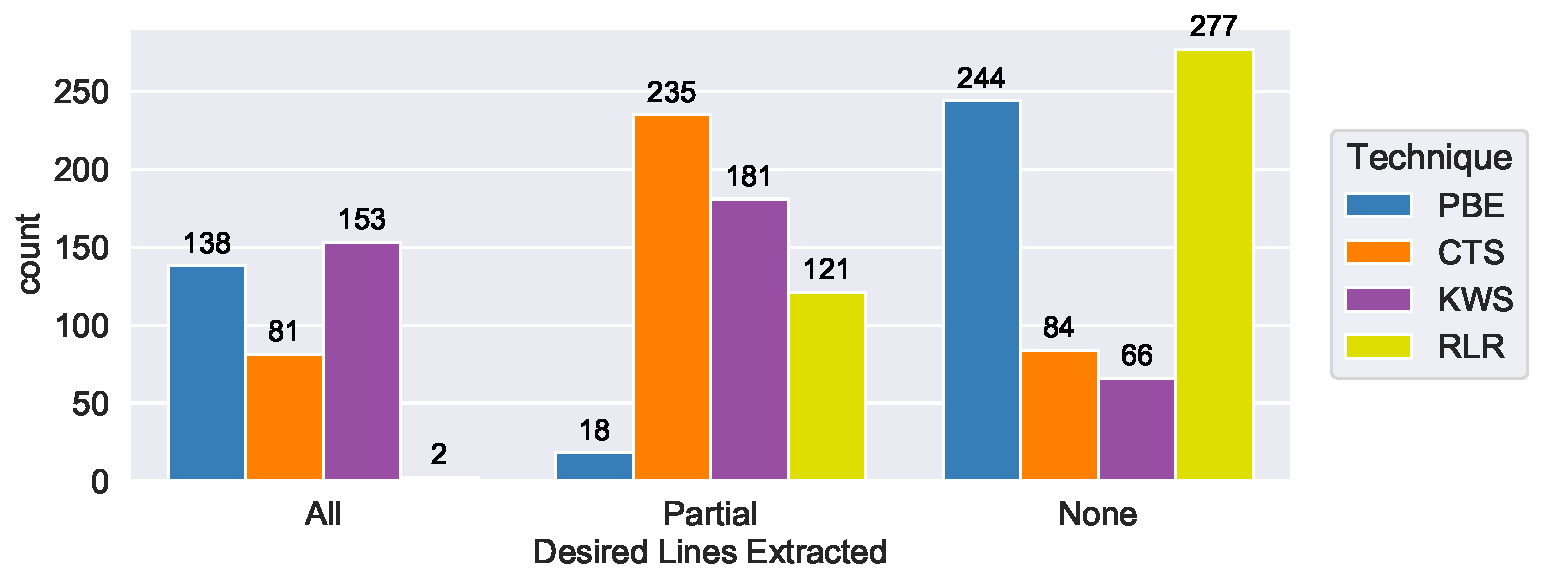
\includegraphics[width=\columnwidth,
		clip]{img/big-study/success-partial-all.pdf}
		\caption{Success of chunk retrievals for all techniques.}
		\label{fig:success-partial-all}
\end{figure}

\begin{figure*}
\centering
    \textbf{PBE, CTS, KWS, and RLR}\par\medskip
\begin{subfigure}[b]{\columnwidth}
		\centering
				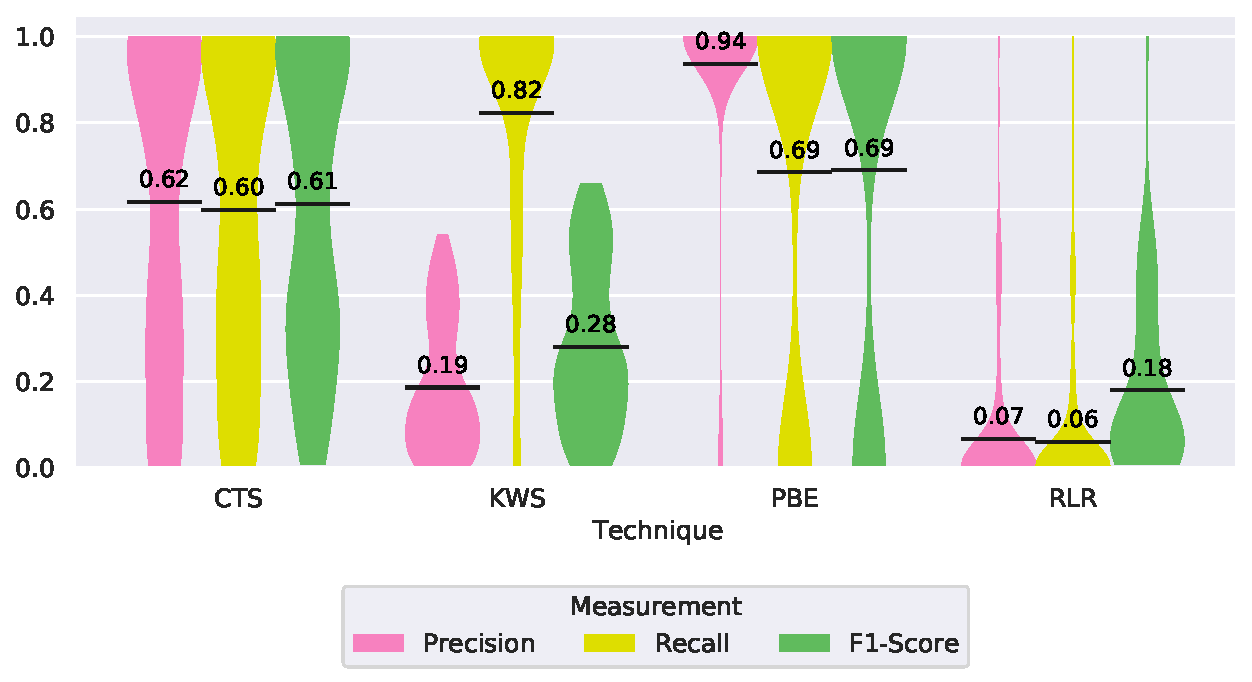
\includegraphics[width=\columnwidth,
				clip]{img/big-study/recall-precision-singlecategory-all.pdf}
		\caption{Training and test examples in 1
		structural category.}
		\label{fig:recall-precision-singlecategory-all}
\end{subfigure}\hspace{\fill}
\begin{subfigure}[b]{\columnwidth}
		\centering
				\centering
		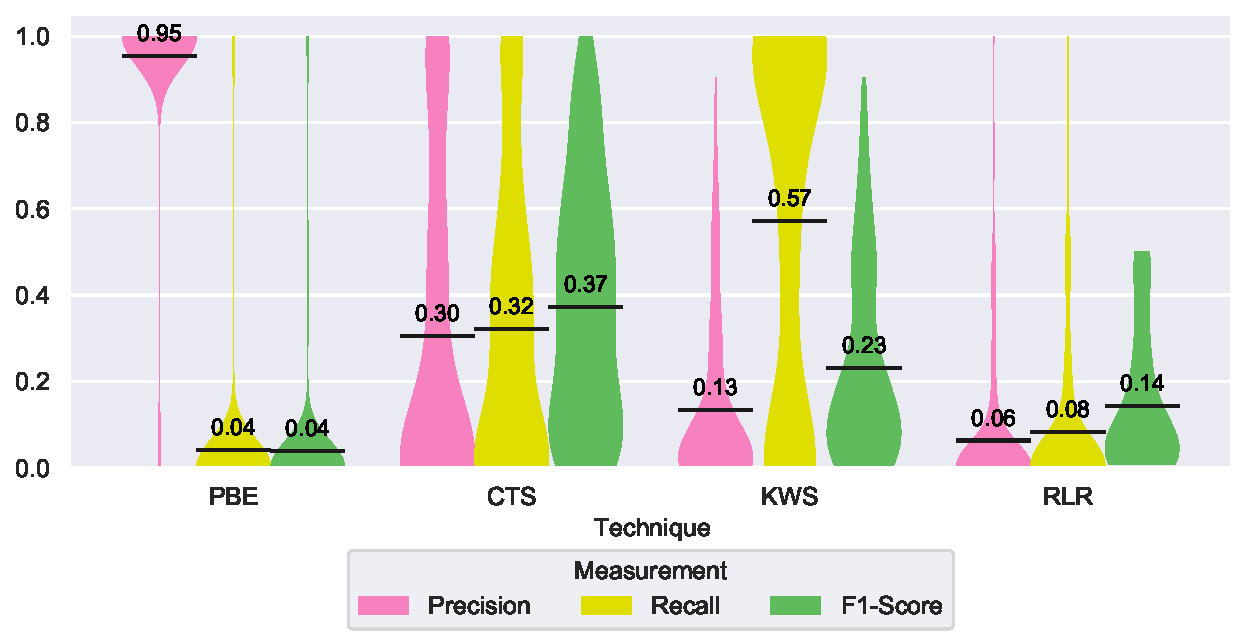
\includegraphics[width=\columnwidth,
		clip]{img/big-study/recall-precision-multicategory-all.pdf}
		\caption{Training and test examples in \textgreater
		1 structural
		category.}
		\label{fig:recall-precision-multicategory-all}
\end{subfigure}
\caption{Precision, recall and F$_{1}$-score of all
techniques compared, split by structural category count.}
\end{figure*}

\section{Discussion}
\label{sec:discussion}

% TODO This sentence is too long and complicated for an intro (and something
% is broken in it, too)
% TODO decision tree -> recommendation schema? You can use the more specific decision
% tree when referencing the figure.
For the interpretation of our study results, we look at each chunk
retrieval technique separately and give recommendations for
which types of input build
logs, available training examples and consumption of the retrieved
output each technique is suited.
Following that, we discuss
which of these criteria should influence the decision to use a certain
chunk retrieval technique most.
Based on our empirical comparison, we present a
decision tree between the three techniques we investigated.

\subsection{Interpretation of Study Results}
% TODO This is bad style. Begin the section by saying what you do in there
% Then at the end, say that you summarized it in Table 3 (or include Table 3
% in the discussion throughout the text.)
\Cref{tab:single-technique-recommendations} summarizes the
recommendations which we discuss
in this section.

\begin{table}[tbp]
\resizebox{\columnwidth}{!}{%
\centering
\begin{tabular}{llll}
  \toprule
  & \textbf{PBE} & \textbf{CTS} & \textbf{KWS} \\
  \midrule
  \textbf{Structural categories} & 1 & less is better & \makecell[l]{best 1 \\
  multiple okay} \\
  \midrule
  \textbf{Training set size} & 2 & no influence & 2 \\
    \midrule
  \textbf{Precision} & \makecell[l]{high \\ (if synthesis succeeds)} & medium &
  low \\
    \midrule
  \textbf{Recall} & \makecell[l]{high \\ (if synthesis succeeds)} & medium &
  high \\
    \midrule
  \makecell[l]{\textbf{Confidence in} \\ \textbf{Output correctness}} & high & low &
  \makecell[l]{low (precision) \\ high (recall)} \\     \midrule 
  \textbf{Output consumer} & program & human & human \\
  \bottomrule
\end{tabular}%
}
\caption{Recommendations for each of the investigated chunk retrieval
techniques.}
\label{tab:single-technique-recommendations}
\end{table}

\subsubsection{Program Synthesis by Example (PBE)}

\noindent
\textbf{Configuration and Input.}
Our study results show that chunk retrieval with PBE gives best
results when the training examples are structurally identical.
This is
because PROSE has difficulty synthesizing OR-based
programs~\cite{mayer2015user}.
PBE is thus suited to retrieve information
chunks that always have the same defining surrounding or internal
structure.
To extract for example the reason a build failed, the log
passage describing the failure would always have to be started and
ended the same way.

When the training examples are of the same structure, one or two
two examples are enough input for PROSE to synthesize a regular
expression program with good recall.
In our study, additional training
examples did not improve the chunk retrieval.
% TODO: Why uncomment the following? Is it not true? I think it is crucial.
% In fact, unless they
% were in some sense redundant, adding training examples above that even
% hindered the applicability of PBE.

\noindent
\textbf{Retrieval Output Usage.}
If the program synthesis succeeds and applying the regular expression
program yields an output, PBE has high precision and recall.
The tool
clearly identifies a failing synthesis or when the regular expression
finds no match on a build log.
Therefore, if PBE produces
an output, the user can have high confidence that it is the desired
output.
This preciseness makes output from PBE chunk retrieval
well-suited for machine consumption and therefore automatic on-ward
processing.

\subsubsection{Common Text Similarity (CTS)}
\noindent
\textbf{Configuration and Input.}
Similar to PBE, chunk retrieval using CTS yields better results the
fewer structural categories are present in the training and test
examples.

The number of training examples had no noticeable influence on
precision or recall in our study.
Information retrieval techniques
like text similarity commonly learn on a higher number of examples
than used for our study.
Future work is needed to investigate how many
examples yield improvements in the chunk retrieval over a single
training example.

\noindent
\textbf{Retrieval Output Usage.}
CTS has good precision and recall on average, though with a high
variation.
This means that the quality of an output by CTS is hard to
determine, which makes it unsuited for automatic  processing and requires
a human to further inspect and interpret the output.
This could include semi-automated procedures such as sending
developers an email with the extracted build failure reason.

\subsubsection{Keyword Search (KWS)}
\noindent
\textbf{Configuration and Input.}
KWS has a higher recall than the two other techniques for multiple
structural categories present in the training and test examples.
This
makes KWS a good technique if there is little prior knowledge of how
the targeted log chunk is represented in the build log.
For the
example of extracting the reason the build failed, KWS is best suited
if a build can fail in various steps logged by different tools and no
pre-categorization of where the build failed is available.

Going from one to two training examples, KWS's recall improves
significantly.
However, further enlarging the training set
does not lead to further improvements.

\noindent
\textbf{Retrieval Output Usage}
While KWS has the highest reca.ll of all three techniques, its
precision is the lowest.
The output of a chunk retrieval with KWS is
well-suited to be read by humans, but ill-suited for consumption by
automated tools.

\begin{figure}[tb]
		\centering
		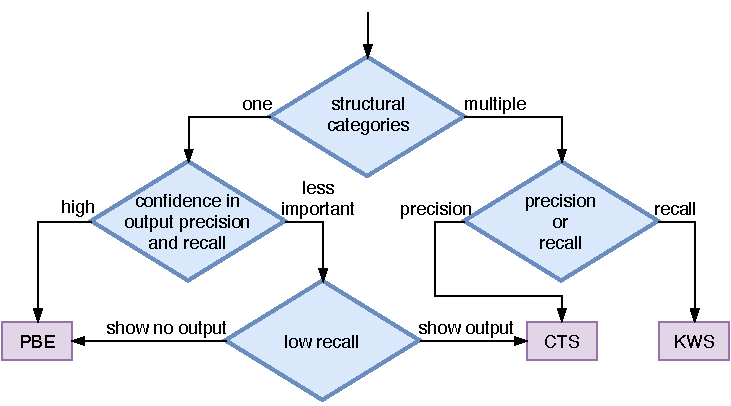
\includegraphics[width=\columnwidth,
		clip]{img/crt-recommendation.pdf}
		\caption{Our preliminary recommendation scheme for chunk
		retrieval techniques.}
		\label{fig:crt-recommendation}
\end{figure}

\subsection{Recommendation of Suitable Techniques}
% TODO Make intor less generic?
After discussing the three chunk retrieval techniques separately we
now want to unify our results into one recommendation scheme.
% TODO Try to inductiviely let the figure emerge from the text, not this
% ``here is the figure; eat it''.
% C: ``How should I do this?''
% Already a better solution would be at the end of this section: We
% summarized these conditions in the decision tree in Fig ...
\Cref{fig:crt-recommendation} presents a decision tree
to answer our second research question;
If researchers or developers want to retrieve chunks from build logs,
they can follow the decision tree to identify the technique
suited best for their use case.
The decision tree is built up of questions
which either lead to more questions or to a leaf node containing a
recommended technique.

% TODO this is too prominent and the style is reserved for RQs ...
% shouldn't it also better be in threats to validity?
\begin{simplebox}[minipage boxed title*=-7cm]{Caveat!}
This is a preliminary hypothesis based on the results
from our comparison study.
The recommendations could therefore be
influenced by idiosyncrasies of our specific implementation of the
chunk retrieval techniques as well as the \emph{LogChunks}
data set.
\end{simplebox}

% TODO for what?
The first and most important aspect are the structural categories.
Are the targeted log chunks always presented in
the same structural way within the build logs? Then the information
chunks in all training examples and the analyzed build log are in the
same structural category.

If the information chunks are from multiple structural categories
and recall is more important than precision we recommend
to use KWS\@.
If precision is more important than recall, we
recommend CTS\@.
We also recommend CTS when the log chunks are
from one structural category, when the user does not require high
confidence in the precision or recall of the outcome and when one
would rather have output with low recall instead of no output at all.
When the representations are from one structural category and the user
wishes high confidence in the correctness of the output or prefers
no output over output with low recall, we recommend PBE\@.

As a final recommendation, one could create a ``super analyzer'' by
combining the different build log analysis techniques studied in this
paper.
Such a super analyzer would likely always first employ PBE
(because of its high accuracy), followed by a combination of CTS and
KWS\@.
Other than initial setup and training time, there is no
downside to this approach if it is implemented in a transparent way to
the underlying technique: the output of the super analyzer could
include from which sub-tool it originated and thus facilitate
automatic on-ward processing or interpretation of the result.


\subsection{Using the Recommendation Scheme}
% TODO Perhaps add introduction from recommendation scheme here?

% TODO this is very nice again, perhaps a tiny bit on the trivial side.
% Do reference Figure 17 more, thoguh
To illustrate how one would use our decision tree to find a suitable
chunk retrieval technique we describe two concrete examples: a software
team
wanting to monitor their build performance and a
researcher investigating why builds fail.

In our first example, a software development team wants to monitor
the performance of the phases within their CI build.
They are using
Travis CI, which measures the duration of build phases and documents
this within the build log.
As all log statements that report timing
measurements are formatted the same way, the targeted log chunks are
from one structural category.
Therefore, the development team can use
PBE to retrieve the duration of a build phase.

In our second example, a researcher wants to investigate whether a small or large group of test cases
causes build failures.
% TODO They?
They gather
CI build logs from various projects.
The task of the researcher is to extract the names of the
failing test cases from each build log.
% TODO They?
When they use our
recommendation scheme to select a chunk retrieval technique, they
first have to estimate how uniform the representation of the failing
test cases is in the investigated build logs.
As the researcher is
covering a wide range of test tools, the
log chunks they target are in various, non-predictable structural
representations.
The next question is whether they value precision
over recall.
As they have to manually inspect the results of both CTS
and KWS, they choose recall over precision to avoid having to inspect
the whole log in case the relevant information chunk was not
retrieved.
Therefore, our decision tree recommends the researcher to use KWS\@.

In case the researcher wants to avoid manually inspecting the
retrieval results, they have to first separate the CI build logs
according to the test tool responsible for logging the test results.
Then the targeted log chunks are from one structural category and they
can use PBE, trained with examples from each test tool separately.

\section{Threats to Validity}
There are several threats to the validity of the conclusions of our
work.


\textbf{Implementation.}
Our results depend on the implementation of the investigated chunk
retrieval techniques and the libraries we used.
Our implementation of
PBE is based on the program synthesis provided by PROSE\@.
The
idiosyncrasies of this framework influence our PBE results.
Other
frameworks similar to PROSE might have somewhat different strengths
and weaknesses.
For example, the need for examples from a single
structural category stems from the fact that PROSE cannot learn
regular expression programs with arbitrary boolean conjunctions and
disjunctions~\cite{mayer2015user}.
PROSE introduced this constraint to
keep the synthesis performance reasonable.
At the same time, this is
clearly a current theoretical challenge of all PBE implementations,
and we therefore attribute it to the technique itself, rather than the
specific implementation.

Our implementation of CTS is dependent on the library
{\tt text2vec}~\cite{text2vec2019webpage}
and the way it splits strings into word tokens.
On the other hand,
{\tt text2vec} is the de-facto standard library to do word embeddings
in R.
We intentionally chose a simple, minimally configured and tuned
approach to compare against.
Tuning the text similarity
meta-parameters more to the specific use case of chunk retrieval from
build logs would yield better chunk retrieval results.

% TODO something like overall, we argue that our implementations and their
% weaknesses stand prototypical for the techniques and tried to limit
% idiosyncrazies as much as possible (give example)

\textbf{Data Set.}
The outcomes of our comparison study are highly dependent on the build
logs from the \emph{LogChunks} data set.
It consists of build
logs from open source projects and therefore it is not clear whether
our results apply to industry projects that use build tools
not popular in open source development.
However, since \emph{LogChunks} covers a wide array of build tools and programming languages,
we believe that our findings do generalize.
We collected build logs from Travis CI.
Yet, the format of the log chunk we chose
for our evaluation is largely independent of Travis CI\@.
This
is because the reason the build failed is described within the build
logs by the tools themselves and not the Travis CI environment.

\textbf{Training Set Size.}
Especially the results for CTS might be influenced by the fact that we
only trained on one to five examples.
We chose this small training set
size as the training examples have to be provided per repository and
we expect a developer to not want to provide more examples than the
small numbers we evaluated on.
The fact that PBE and CTS performed best with already two training
examples shows that our training set size is large enough to
compare the three techniques we presented.

\textbf{Few Samples with Many Structural Categories}
Our comparison study shows fewer measurements with many structural
categories than with one structural category category
(50.25\% one, 33.75\% two, 13.75\% more than two).
This stems from the fact that we investigated the chunk retrieval
techniques on a real-world data set, where there were mostly few
structural categories within one project.
In addition, a third of the measurements were conducted with two
structural categories present and these already showed the negative
effect of the number of structural categories on the performance
of the chunk retrieval techniques.

\section{Future Work}
% TODO Actually, this future work is very, *very* good. It might be
% the best future work I have ever read in an article.
% One idea would be to sell it as such and tie a bit back to our
% first literature sruvey. You can say you give a roadmap to guide
% future research in the field, and sell it in abstract and intro!

There are various future research opportunities based on our work:

\textbf{Systematic Survey of Industry Approaches for Build
Log Analysis.}
Our survey is limited to academic work and articles.
However, handling build logs is a challenge for a wide range of
practitioners as well.
We propose to investigate the methods used in industry to analyze
build logs.
An example is the Jenkins \emph{build-failure-analyzer}
plugin~\cite{jenkins2020failure-analyzer} or automatically
inferred test results in Azure~\cite{azure2020inferred}.

\textbf{Further Analysis of \emph{LogChunks}.}
We created the
\emph{LogChunks} data set \cite{brandt2020logchunks} specifically for
the comparative
study in this paper, though it can be the basis for various further
analyses of build log data.
The keywords, for example, can be
investigated to answer which keywords are used to search for the
reason the build failed within build logs.

\textbf{Cross-Repository Build Log Analysis.}
We trained and
tested each chunk retrieval technique on examples from the same
repository.
We propose to analyze how techniques could be trained
across repositories, building the cornerstones for build
environment-agnostic analysis tools. This has the advantage of creating
a default build log analyzer that would work without any pre-training.

\textbf{Comparison with more Chunk Retrieval Techniques.}
This
paper investigates the three chunk retrieval techniques PBE, CTS and
KWS\@.
Our study design can be reused to evaluate other build log
analysis techniques, such as the diff and information retrieval
approach by Amar et al.~\cite{amar2019mining}.

\textbf{Refinement of Retrieval Quality for each Technique.} We
investigated basic configurations of existing techniques applied to
chunk retrieval from build logs.
In a next step, each of these
techniques could be refined to better approach the domain of build
logs.
The \emph{LogChunks} data set and our study results act as a
baseline to benchmark such technique improvements.
We propose the
following improvements:
\begin{itemize}[leftmargin=0.4cm]
  \item \textbf{Custom Ranking and Tokens for PBE.} The program
  synthesis through PROSE ranks possible programs according to
  what the user most likely intended.
  One could adapt the ranking
  rules provided by the FlashExtract DSL to fit common build log
  chunk retrieval tasks.
  FlashExtract includes special tokens when
  enumerating possible regular expressions.
  One could extend these
  with tokens found in build logs, such as ``-,''
	``=,'' ``ERROR,''
  or ``[OK''.
  \item \textbf{Meta-Parameter Optimization for CTS.} Information
  retrieval techniques have various meta-parameters which can be
  optimized for the specific use
  case~\cite{panichella2016parameterizing}.
  We propose to further
  investigate improvements in preprocessing of the log text, in
  tokenization of the log lines into terms and in stop words
  lists.
\end{itemize}

\textbf{Usability Analysis of Chunk Retrieval Output.}
Our
analysis of the output produced by the chunk retrieval focuses on
precision and recall.
A next step could be to investigate how useful these
outputs really are to developers through controlled experiments or user studies.

\section{Conclusion}
\label{sec:conclusion-fw}
% TODO conclusion should be a bit longer and a little bit more in
% detail. Mention general accuracy measures (techniques performed
% up to in F1 score, which is x times better than RLR)
% TODO could also mention future research here: Finally, we gave an
% outline to guide future research efforts in the area of build log
% analysis.
The goal of this paper was to support researchers and developers in
their decision on how to analyze build logs.
To this end, we conducted a systematic mapping study to uncover the
state-of-research on build log analysis.
We implemented	three promising chunk retrieval techniques and
compared their performance on the \emph{LogChunks} data set.
Our results show that the structural
representation of the targeted information in the build logs is the
main factor to consider when choosing a suitable technique.
Secondary
factors are the desired confidence into recall and precision of the
produced output and whether precision or recall is more important for
the task at hand.

